\chapter{Implementation and Evaluation}
\label{implementation}

This chapter presents the algorithm for checking composition; the implementation of activations, heaps, and (two) schedulers; and I/O facilities for an interpreter designed for the \rcgo programming language presented in Chapter~\ref{language}.

\section{Interpreter Organization and Implementation}
\label{interpreter}

The interpreter consists of a scanner, a parser, a sequence of semantic checks, a code generation phase, composition checks, and an execution phase.
The interpreter is implemented in C++.
Flex and Bison were used to implement the scanner and parser, respectively.
The semantic checks include type checking and enforcement of intrinsic and dereference mutability as set forth in Chapter~\ref{language}.
The code generation phase converts the AST into a tree of stack operations.
The composition check synthesizes transactions and checks them for soundness (Section~\ref{sound_composition}).
The execution phase begins by initializing component instances by calling the initializer associated with each instance.
The scheduler then proceeds by selecting and executing transactions according to weak fairness (Section~\ref{scheduler}).
The scheduler implementations use the POSIX threads (pthreads) library for concurrent execution and synchronization.
The code is available on GitHub\footnote{https://github.com/jrw972/rc}.

\section{Enforcing Sound Composition}
\label{sound_composition}

\subsection{Background}

This section outlines the algorithm for checking the composition semantics of reactive components.
As described in Chapter~\ref{model}, one of the goals for the reactive component model is to facilitate the construction of complex reactive systems through composition.
The composition semantics of reactive components overcome limitations of I/O automata and UNITY but introduce concurrency hazards that may result in systems whose behavior is not well defined.
Two key hazards to be avoided are non-deterministic transactions arising from the same state being updated by multiple transitions within a transaction, and recursive transactions arising from cycles in composition.
The goal of the composition check is to determine whether a system is free of these hazards.

Checking for sound composition is a holistic problem.
Ports facilitate third-party composition by being opaque, meaning that the action or reaction activating a port cannot know or care about the state transitions executed as a result of activating the port.
The state involved in a transaction is not known until the components are instantiated and the ports bound.
Thus, checking for sound composition requires a reasonably complete understanding of the system.
To this end, the algorithm described in this section leverages the static system assumption\footnote{I.e., that all components are known \emph{a priori} and no components are added or removed from the system at run-time.}.
We leave relaxing the static system assumption, which will require extending the model and proposed checking algorithm, to future work.

The language semantics of Chapter~\ref{model} entail a number of assumptions that allow composition checking to be formulated as a set of simple graph- and set-theoretic problems.
Activation statements are limited to the bodies of actions and reactions and port calls are limited to activation statements.
Activation statements terminate the execution of an action or reaction, meaning at most one will be called per action or reaction body.
Thus, a transaction can be viewed as a directed graph where each node is an action or reaction and edges indicate that the source action or reaction activates the target reaction.
With this graph in place, the state involved in a transaction can be deduced by treating the component instances as proxies for their state variables by creating sets of instances and evaluating the sets for compatibility.

\subsection{Algorithm Sketch}

\paragraph{Enumerate instances and ports.}
The first step to analyzing composition is to enumerate the components in the system using the static system assumption.
The top-level components are given by the declared instances.
Sub-components are enumerated by recursively instantiating fields that are also components.
Let $I$ denote the set of component instances.
Fields that are ports are also enumerated.
Let $S$ denote the set of push ports and $L$ denote the set of pull ports.

\paragraph{Enumerate bindings.}
Let $i$ be a component instance of type $c$.
Associated with $c$ is a set of binders $B$.
Each binder $b \in B$ is evaluated for $i$ to create a set of bindings.
A binding either binds a push port to a reaction or a getter to a pull port.
Let $R$ denote the set of reactions and $G$ denote the set of getters.
The result of enumerating the bindings is two functions (look-up tables).
The function $\mathit{reactions}: S \to \{ R \}$ maps a push port to a set of reactions.
The function $\mathit{getters}: L \to \{ G \}$ maps a pull port to a set of getters.

\paragraph{Check bindings.}
Inverting $\mathit{reactions}$ yields a function that maps a reaction to a set of push ports, $\mathit{reactions}^{-1}: R \to \{ S \}$.
The $\mathit{reactions}^{-1}$ function is used to ensure that a reaction either is bound to one push port or is not bound:
\begin{displaymath}
\forall r \in R : |\mathit{reactions}^{-1} (r)| \leq 1
\end{displaymath}
The $\mathit{getters}$ function is used to ensure that a pull port is bound to exactly one getter:
\begin{displaymath}
\forall l \in L : |\mathit{getters} (l)| = 1
\end{displaymath}

\paragraph{Enumerate transactions.}
Let $i$ be a component instance of type $c$.
Associated with $c$ is a set of actions $A$.
Each action $a \in A$ is evaluated for $i$ to create a transaction.
A \emph{transaction} is a directed graph constructed as follows, as the example in Figure~\ref{transaction} illustrates:
\begin{enumerate}
\item The root is the action $a$.
\item The descendants of the root are the activations in $a$ and the pull ports and the getters used in the immutable phase.
\item The descendants of the pull ports are the getters bound to the pull ports given by $\mathit{getters}$.
\item The descendants of the activations are the push ports named in each activation.
\item The descendants of the push ports are the reactions bound to the push ports given by $\mathit{reactions}$.
\item This process is then repeated for each reaction and getter.
\end{enumerate}

\begin{figure}
\centering
%%\resizebox{\textwidth}{!}{%
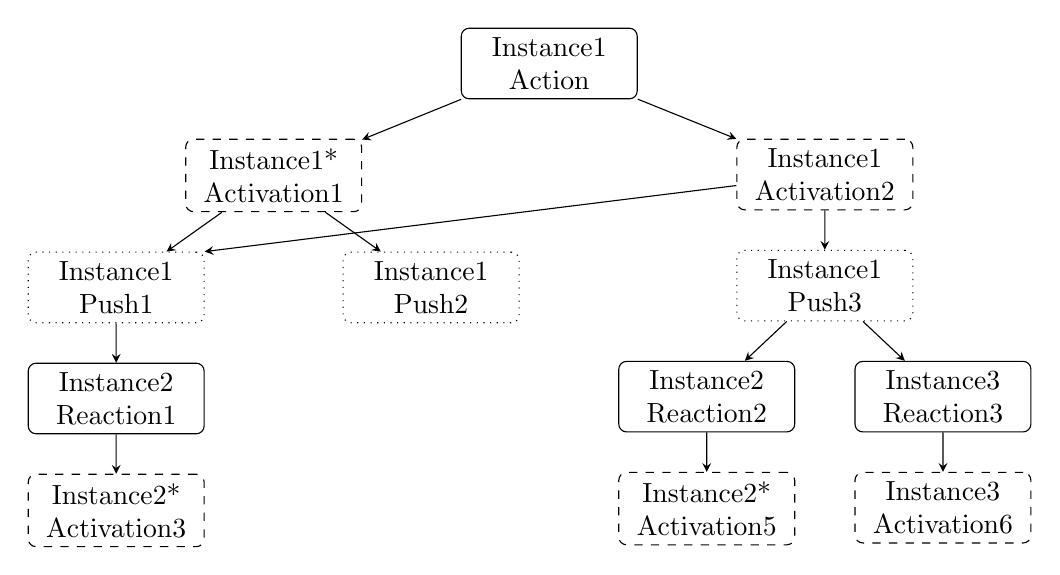
\begin{tikzpicture}[
    arrowstyle/.style={draw, -stealth},
    edge from parent/.style={draw, -stealth},
    reaction/.style={rectangle, draw, rounded corners=1mm, text width=2cm,
        text centered, anchor=north},
    activation/.style={rectangle, draw, rounded corners=1mm, dashed, text width=2cm,
        text centered, anchor=north},
    push/.style={rectangle, draw, rounded corners=1mm, dotted, text width=2cm,
        text centered, anchor=north},
    level 1/.style={sibling distance=7.0cm},
    level 2/.style={sibling distance=4.0cm},
    level 3/.style={sibling distance=3.0cm},
    level distance=0.5cm, growth parent anchor=south
]
\node (Action) [reaction] {Instance1 Action}
  child {
    node (Activation01) [activation] {Instance1* Activation1}
    child {
      node (Push01) [push] {Instance1 Push1}
      child {
        node (Rection01) [reaction] {Instance2 Reaction1}
        child {
          node (Activation03) [activation] {Instance2* Activation3}
        }
      }
    }
    child {
      node (Push02) [push] {Instance1 Push2}
    }
  }
  child {
    node (Activation02) [activation] {Instance1 Activation2}
    child {
      node (Push03) [push] {Instance1 Push3}
      child {
        node (Rection02) [reaction] {Instance2 Reaction2}
        child {
          node (Activation04) [activation] {Instance2* Activation5}
        }
      }
      child {
        node (Rection03) [reaction] {Instance3 Reaction3}
        child {
          node (Activation05) [activation] {Instance3 Activation6}
        }
      }
    }
  }
;

\draw[arrowstyle] (Activation02) -- (Push01.north east);

\end{tikzpicture}
%%}%
\caption{Example transaction\label{transaction}}
\end{figure}

A recursive transaction is formed when a reaction activates itself through the set of bindings or a getter calls itself, which appears as a cycle in the transaction graph.
The interpreter contains an implementation of Tarjan's algorithm~\cite{tarjan1976} to detect cycles.

A non-deterministic transaction occurs when the same state is manipulated by multiple transitions.
Thus, the interpreter must determine what state is manipulated in a transaction to determine if the constituent transitions are compatible.
The interpreter uses a component instance as a proxy for its state variables and determines how the state is accessed in each transition.
The possible access patterns include:
\begin{description}
  \item[Write] in which at least one state variable may be mutated (* in figure~\ref{transaction})
  \item[Read] in which at least one state variable is accessed but no state variables are mutated
  \item[None] in which no state variables are accessed
\end{description}
The current implementation uses a conservative static analysis of the body of an activation statement to determine if the activation mutates the state of the component.
For composition analysis, state variable access need only be determined for the mutable phase.
However, also performing a similar analysis for the immutable phase and precondition provides a complete description of state access in a transaction, which is used by multi-threaded schedulers to determine which transactions can be executed in parallel.

The check for non-deterministic transactions continues by confirming that all possible executions of a transaction are deterministic in two steps.
First, two \emph{access sets} are computed for each node in the transaction.
The first access set describes what state is accessed in the immutable phase, while the second set describes what state is accessed in the mutable phase.
Let $W = \{ \mathit{Read}, \mathit{Write} \}$ be the set of possible access patterns.
Each element in an access set $h \in H$ is a pair $(i,w)$ where $i \in I$ and $w \in W$.
Let $\mathit{inst}: A \cup R \cup G \to I$ be a function that maps an action, reaction, or getter to the corresponding instance.
The immutable phase access sets are computed as follows:
\begin{itemize}
  \item For an action, reaction, or getter denoted as $x$ with instance $i = \mathit{inst}(x)$ that reads the state of $i$, the immutable phase access set is the union of the immutable phase access sets of its children and the set $\{ (i, \mathit{Read}) \}$.
  \item Otherwise, the immutable phase access set is just the union of the immutable phase access sets of its children.
\end{itemize}
The mutable phase access sets are computed as follows:
\begin{itemize}
  \item If the node is not an activation, or is an activation that does not access the state of the instance, then the mutable phase access set is the union of the mutable phase access sets of its children.
  \item Otherwise, the node is an activation belonging to instance $i \in I$ with access $w \in W$ and the mutable phase access set is the union of the mutable phase access sets of its children and $\{ (i, w) \}$.
\end{itemize}
The access sets for the root of a transaction describe how state may be accessed during each phase of the transaction.
An analysis similar to the immutable phase analysis may be applied to the precondition.
All access pairs in the precondition and immutable phase access sets have $\mathit{Read}$ access.
Access pairs in the mutable phase access sets may either have $\mathit{Read}$ or $\mathit{Write}$ access.
Activation statements that do nothing but log the state of a component are a common example of mutable phase access pairs with $\mathit{Read}$ access.

\begin{figure}
\centering
%%\resizebox{\textwidth}{!}{%
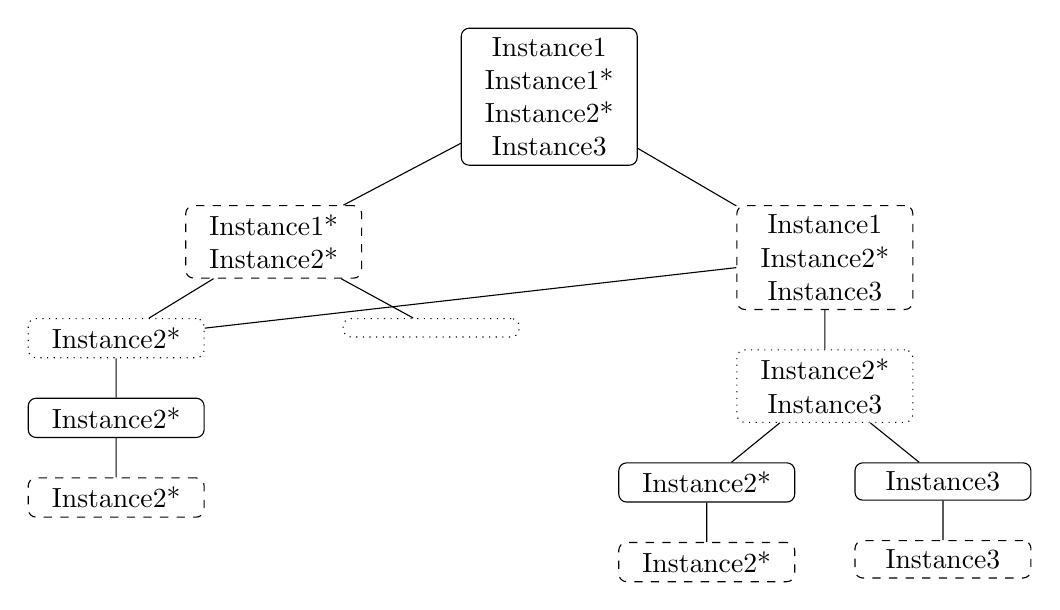
\begin{tikzpicture}[
    reaction/.style={rectangle, draw, rounded corners=1mm, text width=2cm,
        text centered, anchor=north},
    activation/.style={rectangle, draw, rounded corners=1mm, dashed, text width=2cm,
        text centered, anchor=north},
    push/.style={rectangle, draw, rounded corners=1mm, dotted, text width=2cm,
        text centered, anchor=north},
    level 1/.style={sibling distance=7.0cm},
    level 2/.style={sibling distance=4.0cm},
    level 3/.style={sibling distance=3.0cm},
    level distance=0.5cm, growth parent anchor=south
]
\node (Action) [reaction] {Instance1 Instance1* Instance2* Instance3}
  child {
    node (Activation01) [activation] {Instance1* Instance2*}
    child {
      node (Push01) [push] {Instance2*}
      child {
        node (Rection01) [reaction] {Instance2*}
        child {
          node (Activation03) [activation] {Instance2*}
        }
      }
    }
    child {
      node (Push02) [push] {}
    }
  }
  child {
    node (Activation02) [activation] {Instance1 Instance2* Instance3}
    child {
      node (Push03) [push] {Instance2* Instance3}
      child {
        node (Rection02) [reaction] {Instance2*}
        child {
          node (Activation04) [activation] {Instance2*}
        }
      }
      child {
        node (Rection03) [reaction] {Instance3}
        child {
          node (Activation05) [activation] {Instance3}
        }
      }
    }
  }
;

\draw (Activation02) -- (Push01);

\end{tikzpicture}
%%}%
\caption{Example mutable phase access set calculation\label{access_sets}}
\end{figure}

Figure~\ref{access_sets} shows the mutable phase access set calculation for the transaction illustrated in Figure~\ref{transaction}.
The root shows that Instance1 does not change in at least one activation (Instance1) and may change in at least one activation (Instance1*), that Instance2 may change in every activation (Instance2*), and that Instance3 is read-only in this transaction (Instance3).
The empty node in Figure~\ref{access_sets} comes from an unbound push port.

The second step for detecting a non-deterministic transaction is to verify that a mutated instance appears in at most one child node access set for the activation and push port nodes.
Let $\mathit{race}: \{ H \} \times \{ H \} \to \mathcal{B}$ be a predicate that indicates a data race between two access sets.
This function is defined as follows:
\begin{multline}
  \mathit{race} (H_1, H_2) = \\
  (\exists i : (i, \mathit{Write}) \in H_1 \land (i, x) \in H_2) \lor
  (\exists j : (j, \mathit{Write}) \in H_2 \land (j, y) \in H_1)
\end{multline}
This is, a component that changes state in one access set may not appear in the other access set.
The $\mathit{race}$ predicate is computed for each pair of child mutable phase access sets in activation and push port nodes.
This check succeeds everywhere but Activation2 in Figures~\ref{transaction}~and~\ref{access_sets}, as Instance2* appears in both children.
The activation and push port nodes represent activities that will be performed together.
That is, once control passes to an activation statement, all push ports and their bound reactions are activated.
In contrast, activations (as children of action and reaction nodes) represent mutually exclusive alternatives:  at most one activation statement is executed per action/reaction body.
Thus, a mutated instance appearing in two or more children of an activation node or push port node indicates that the state of a component may be mutated in disparate ways leading to a non-deterministic transaction.

\paragraph{Complexity.}
Maintaining appropriate forward and reverse hash maps of the bindings allows the binding check to be performed in $O(N)$ time where $N$ is the number of ports in the system.
Similarly, the construction of a transaction graph can be performed in $O(|N| + |V|)$ time where $|N|$ is the number of nodes in the transaction and $|V|$ is the number of edges.
Proving that a transaction is acyclic can be performed in $O(|N| + |V|)$ time where $|N|$ is the number of nodes and $|V|$ is the number of edges.

A loose upper-bound on the complexity of the access set calculations for the non-determinism check is $O(k |N|^2 \log (|N|))$ where $|N|$ represents the number of nodes in a transaction and $k$ represents the maximum branching factor in the transaction.
The size of the access set for the root is $|N|$.
Assuming a naive set implementation, the complexity of computing the access set for the root is $O(|N| \log (|N|))$.
This must be repeated $k$ times for all nodes in the graph resulting in an overall complexity of $O(k |N|^2 \log (|N|))$.

A loose upper-bound on the complexity of the compatibility check is also $O(k |N|^2 \log (|N|))$.
Assume that the size of the access set at each node is $|N|$.
A tree-based set lookup can be performed in $O(\log(|N|))$ time.
The lookup must be performed $k |N|$ times by the parent.
The lookup must repeated for each of the $|N|$ nodes for a combined complexity of $O(k |N|^2 \log (|N|))$.

The complexity of these algorithms has not presented a problem in practice as most of the systems we have implemented have small numbers for $|N|$, $|V|$, and $k$.

\section{Activations}
\label{activations}

When executing a transaction, the run-time must execute the immutable phase of all implied state transitions before executing any of the mutable phases.
To accomplish this, the run-time uses a novel calling convention to create a list of deferred contexts and statements that represent the mutable phase of each state transition.
The immutable phase constructs the list and the mutable phase processes the list.
To present the calling convention, we first present some details about the run-time such as the ordinary calling convention and push ports.
We then describe the behavior of the calling convention and explain it using an illustrative example.

\paragraph{Ordinary calling convention.}
The ordinary call mechanism in the run-time is similar to the C-decl calling convention.
It assumes the existence of an \emph{instruction pointer}, which contains the address of the currently executing instruction, and a \emph{base pointer} that points to a location in the stack, which can be offset to access arguments and local variables.
A ordinary call in the language is accomplished through the following sequence:
\begin{enumerate}
\item (Caller) Push arguments onto the stack, left to right.
\item (Caller) Push the instruction pointer onto the stack and transfer control to the body of the function, method, action, reaction, getter, or initializer.
\item (Callee) Push the base pointer onto the stack and set the base pointer to the top of the stack.
\item (Callee) Reserve space on the stack for local variables.
\item (Callee) Execute the body of the function, method, etc.
\item (Callee) Pop the stack, pop and restore the base pointer, pop and restore the instruction pointer.
\item (Caller) Pop the arguments.
\end{enumerate}
The major difference between this calling convention and C-decl is that the arguments are pushed in the opposite order to match the semantics of Go.
The collection of arguments, previous instruction pointer, previous base pointer, and reserved space is called a \emph{stack frame} (or \emph{call frame}).
Figure~\ref{frame} shows the layout of a normal stack frame.
For this presentation, we assume that the stack grows down, i.e., the previous base pointer has a lower address in memory than the previous instruction pointer.

\begin{figure}
\centering
\resizebox{.5\textwidth}{!}{%
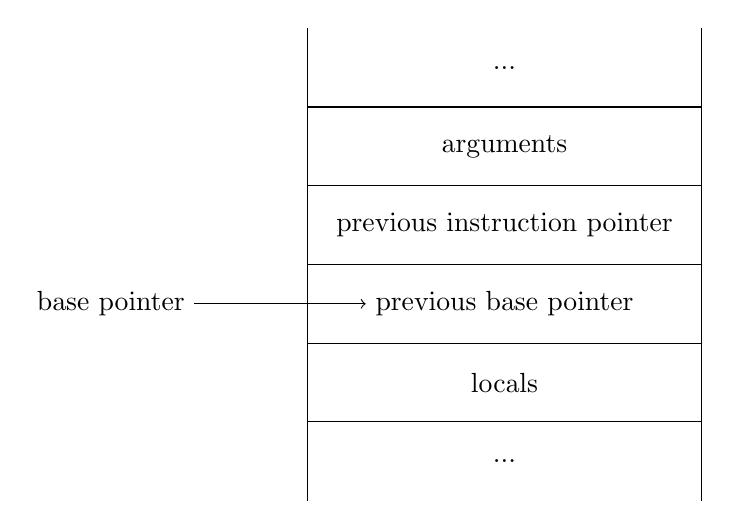
\begin{tikzpicture}
%% component boundary

\draw (0,1) -- (0,7);
\draw (5,1) -- (5,7);

\node at (2.5, 6.5) { ... };
\draw (0,6) -- (5,6);
\node at (2.5, 5.5) { arguments };
\draw (0,5) -- (5,5);
\node at (2.5, 4.5) { previous instruction pointer };
\draw (0,4) -- (5,4);
\node (pbp) at (2.5, 3.5) { previous base pointer };
\draw (0,3) -- (5,3);
\node at (2.5, 2.5) { locals };
\draw (0,2) -- (5,2);
\node at (2.5, 1.5) { ... };

\node (bp) at (-2.5, 3.5) { base pointer };
\draw[->] (bp) -- (pbp);

\end{tikzpicture}
}%
\caption{Diagram of a stack frame\label{frame}.  The stack is depicted as growing down.}
\end{figure}

\paragraph{Push ports.}
A push port is a field in a component, which is implemented as a pointer to a linked list that contains the component pointer/reaction pairs that are bound to the push port.
The run-time populates each push port before execution begins.

\paragraph{Synchronized two-phase calling convention.}
As previously stated, the execution of an activation statement is split into an immutable phase and a mutable phase.
To prepare for the mutable phase, the immutable phase must preserve the stack frame (context) of the action or reaction that executes an activation statement and must record which activation statement was executed so that the same activation can be resumed in the mutable phase.
To accomplish this, we devised a \emph{synchronized two-phase calling convention}, which is used to execute activation statements during the immutable phase.

Recall that activation statements may only appear in actions and reactions.
After executing the immutable phase of an activation statement in a reaction, control must be returned to the calling activation statement so that it may activate other push ports.
After executing the immutable phase of an activation statement in an action, control must be returned to the run-time to begin the mutable phase.

In the ordinary calling convention, the call frame for the reaction would be popped, control would be returned to the caller, and the arguments would be popped.
To preserve the call frame for use during the mutable phase, however, the activation statement returns control to the caller without popping the frame and the caller does not pop the arguments.
Thus, the complete frame for the reaction is preserved on the stack.

Each deferred call frame is added to a list to make it available in the mutable phase.
Let $head$ be a variable containing a pointer, initially nil, which will serve as the head of a linked list.
Before the activation statement returns from the immutable phase, it sets the previous base pointer in the call frame to the value of $head$ and updates head to be the current base pointer which inserts the call frame into the list.
The run-time can iterate over the elements of the list by following the previous base pointer to access all of the call frames that are needed for the mutable phase.
If the list is empty ($head$ is nil), then no activation statement was executed and the mutable phase may be skipped.

The final piece of information that must be recorded is the body of the activation statement so that it is accessible in the mutable phase.
Before returning from the immutable phase, the activation statement records the body of the activation statement in the previous instruction pointer slot of the call frame.
It is safe to use the previous instruction pointer because it is not used beyond the immediate return.
Furthermore, it is at a fixed location, which allows it to be accessed in any deferred call frame.

The synchronized two-phase calling convention is used when executing an activation statement and proceeds as follows:
\begin{enumerate}
\item Save the previous base pointer of the current stack frame in $bp$.
\item Set the previous base pointer of the current stack frame to the value of $head$.
\item Set $head$ to the value of the base pointer.
\item Save the previous instruction pointer of the current stack frame in $ip$.
\item Set the previous instruction pointer of the current stack frame to the body of the activation statement.
\item For each push port in the port call list:
  \begin{enumerate}
  \item Push the arguments to the push port onto the stack.\label{step1}
  \item For each component pointer/reaction pair in the push port:
    \begin{enumerate}
    \item Push the component pointer onto the stack.
    \item Copy the arguments prepared in~\ref{step1} onto the stack.
    \item Call the reaction.
    \end{enumerate}
  \end{enumerate}
\item Set the base pointer to the value of $bp$ and return control to the address in $ip$.
\end{enumerate}

The synchronized two-phase calling convention evaluates the arguments to a push port once and passes a copy to each bound reaction.
One alternative is to evaluate the arguments for each bound reaction.
This means that the arguments may not be evaluated (i.e., the push port is not bound to any reactions) or may be evaluated multiple times.
If the arguments contain an expression with side-effects, then the behavior of the code becomes dependent on composition.
While this may be desirable in some cases, we opted for making a port call resemble an ordinary function call as much as possible.
This sentiment also influenced our decision to pass a copy of the arguments to each reaction as opposed to reusing the same set of prepared arguments.
Since each reaction starts with a copy of the arguments, it is free to manipulate them as allowed by the semantics of Go.
Furthermore, the arguments are available in the mutable phase which obviates the need to make local copies of arguments.
This approach assumes that copying arguments does not generate significant overhead.

%% After an activation statement calls the last push port, it makes temporary copies of the instruction pointer and base pointer of the caller.
%% It may then safely overwrite the base pointer to insert itself into the list of mutable phase call frames and it may safely overwrite the instruction pointer with the body of the activation statement.

A major caveat when using the synchronized two-phase calling convention is that it must be assumed that the stack pointer changes when calling a push port.
To illustrate why this is an issue, consider the case when a caller wishes to preserve the contents of a register.
One strategy is to push the contents of the register onto the stack, perform the call, and then pop the value from the stack into the register.
After calling a push port, the caller may no longer assume that the previous value of the register is at the top of the stack.
An easy work-around is to allocate local variables, i.e., variables whose addresses are relative to the base pointer instead of the stack pointer, for saving temporary values that must persist across a push port call.
In the same way, the variables used to iterate over the list of component/reaction pairs in a push port should be allocated as local variables so that they may survive the calls to the reactions.

\paragraph{Mutable phase.}
The mutable phase consists of executing all of the deferred activation statements.
The algorithm for doing so is as follows:
\begin{enumerate}
\item If the value of $head$ is nil, stop.  Otherwise, set the base pointer to the value in $head$.
\item Transfer control to the instruction indicated by the previous instruction pointer\label{transfer}.  Execution continues until the body of the activation statement (implicitly or explicitly) returns.
\item If the previous base pointer is nil, stop.  Otherwise, set the base pointer to the previous base pointer and go to \ref{transfer}.
\end{enumerate}

The algorithm iterates over the list of deferred call frames accessible through $head$.
The last element in the list is indicated by a previous base pointer that is nil.
Control is transferred to the previous instruction pointer which contains the body of the activation statement.

\begin{figure}
\centering
\resizebox{.75\textwidth}{!}{%
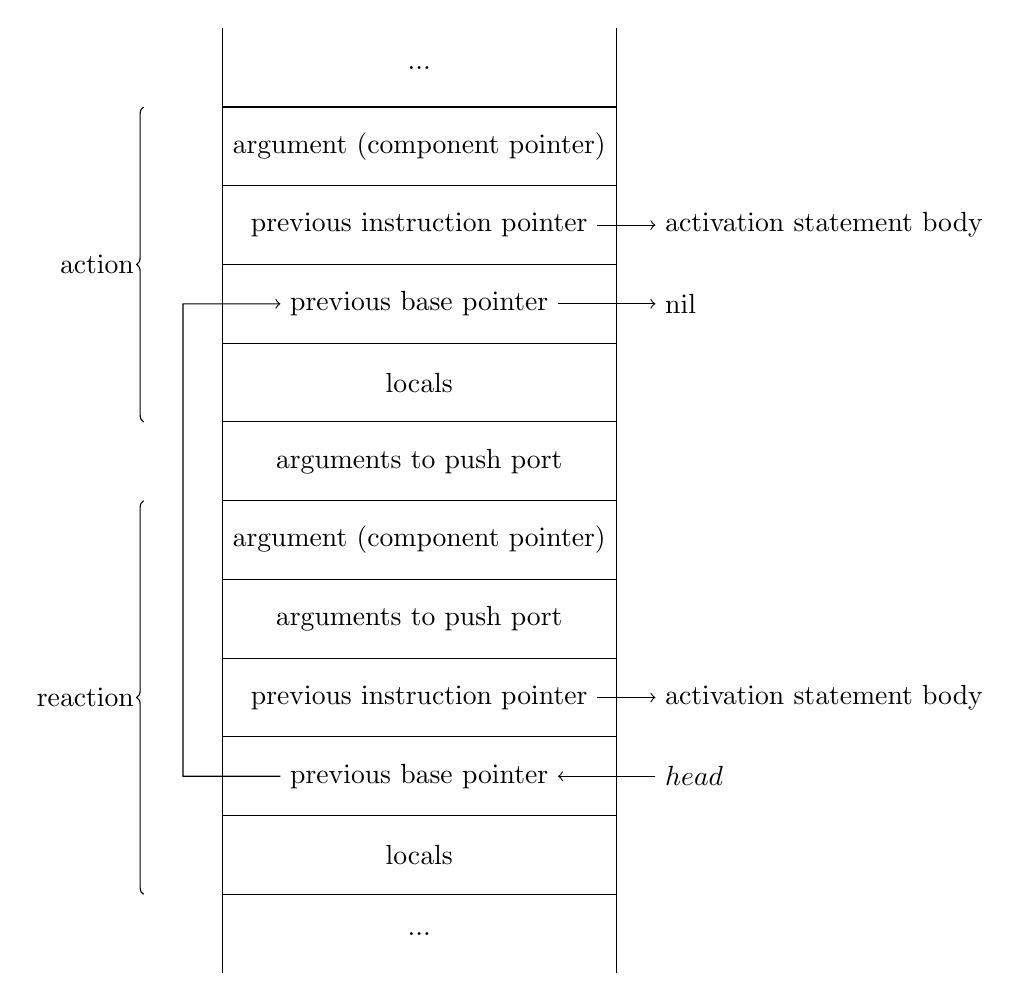
\begin{tikzpicture}
%% component boundary

\draw (0,-5) -- (0,7);
\draw (5,-5) -- (5,7);

\node at (2.5, 6.5) { ... };
\draw (0,6) -- (5,6);
\node at (2.5, 5.5) { argument (component pointer) };
\draw (0,5) -- (5,5);
\node (pip1) at (2.5, 4.5) { previous instruction pointer };
\draw (0,4) -- (5,4);
\node (pbp1) at (2.5, 3.5) { previous base pointer };
\draw (0,3) -- (5,3);
\node at (2.5, 2.5) { locals };
\draw (0,2) -- (5,2);
\node at (2.5, 1.5) { arguments to push port };
\draw (0,1) -- (5,1);
\node at (2.5, .5) { argument (component pointer) };
\draw (0,0) -- (5,0);
\node at (2.5, -.5) { arguments to push port };
\draw (0,-1) -- (5,-1);
\node (pip2) at (2.5, -1.5) { previous instruction pointer };
\draw (0,-2) -- (5,-2);
\node (pbp2) at (2.5, -2.5) { previous base pointer };
\draw (0,-3) -- (5,-3);
\node at (2.5, -3.5) { locals };
\draw (0,-4) -- (5,-4);
\node at (2.5, -4.5) { ... };

\node[anchor=west] (as1) at (5.5, 4.5) { activation statement body };
\draw[->] (pip1) -- (as1);
\node[anchor=west] (as2) at (5.5, -1.5) { activation statement body };
\draw[->] (pip2) -- (as2);

\draw[->] (pbp2) -- ++(-3,0) -- ++(0,6) -- (pbp1);

\node[anchor=west] (nil) at (5.5, 3.5) { nil };
\draw[->] (pbp1) -- (nil);

\node[anchor=west] (head) at (5.5, -2.5) { $head$ };
\draw[->] (head) -- (pbp2);

\draw[decorate,decoration={brace}] (-1,2) -- (-1,6) node[anchor=east,midway] { action };

\draw[decorate,decoration={brace}] (-1,-4) -- (-1,1) node[anchor=east,midway] { reaction };

\end{tikzpicture}
}%
\caption{Diagram of the stack after the immutable phase when an action activates a single reaction.\label{activation_ex_1}}
\end{figure}

\paragraph{Example:  one action, one reaction.}
Suppose an action activates a single push port that is bound to a single reaction and the reaction has a single activation that does not activate any push ports.
Figure~\ref{activation_ex_1} shows a diagram of the stack after the immutable phase for this scenario.
The stack contains two frames, one corresponding to the action and one corresponding to the reaction.
The $head$ variable points to the reaction frame which in turn points to the action frame using the previous base pointer slot.
The action frame points to nil indicating that it is the last frame in the list.
The previous instruction pointers point to the bodies of the activation statements.
Between the frames are the push port arguments which are duplicated for the call to the reaction.
If the push port had been bound to multiple reactions, then the reaction portion of the diagram would be replicated to match the number of bound reactions.
If multiple push ports were activated by the activation statement, then additional push port arguments and reactions would appear on the stack.

\paragraph{Calling convention efficiency.}
The synchronized two-phase calling convention has the potential to be as efficient as a function or method call.
The proposed calling convention can be implemented directly on modern hardware architectures like x86 and x86\_64, which contain all of the registers and instructions necessary to support the synchronized two-phase calling convention.
The synchronized two-phase calling convention relies solely on the stack which means that the underlying operating system must set up the stack, back it with memory pages, etc.
More importantly, it avoids the overhead of heap allocation.
Port calls resemble virtual method calls in that the reactions must be looked up before they can be executed.
However, this lookup could be avoided by inlining the body of each reaction using the substitutional equivalence property.
This could be performed prior to execution or during execution using just-in-time compilation techniques.
We leave the application of these technique as future work.

\section{Heaps}
\label{heaps}

In this section, we describe the implementation of the heap data type introduced in chapter~\ref{language} and our approach to garbage collection.
Our approach to implementing dynamic memory allocation and garbage collection was shaped by the independence of state required by the semantics of reactive components.
Thus, instead of relying on a single global heap, the implementation contains a heap for each component that can be garbage collected independently of the others.
This independence allows garbage collection to be performed concurrently with other activities using simple, single-threaded algorithms.

\paragraph{Slots and blocks.}
A \emph{slot} is the smallest unit of memory that can be dynamically allocated.
Typically, a slot is the size of two pointers.
A \emph{block} is an extent of memory and a set of bits indicating the allocation status of each slot in the extent.
The status bits indicate if a slot is allocated, if a slot is the beginning of an object, and if the slot has been marked by the mark-and-sweep algorithm.
Blocks also contain left and right pointers that allow them to be formed into a binary tree ordered by the address of the extent.

\paragraph{Mark-and-sweep garbage collection.}
We implemented a simple mark-and-sweep algorithm to collect garbage in a tree of blocks.
The core of the marking phase involves scanning extents for pointers to objects.
When the algorithm comes across a slot that is allocated, marked, and which contains a pointer-sized value that points to a location in the tree of blocks that is also allocated, it marks the object indicated by the pointer.
The algorithm is bootstrapped by marking all slots in a designated root object.
The algorithm repeatedly scans the extents in the tree of blocks until no new marks can be added.
At this point, the sweep phase resets the allocated bit for all slots that are allocated but not marked and resets the marked bit for the next run of the algorithm.
A block that is not marked, meaning that none of its slots were marked, is removed from the tree of blocks and deallocated.

\paragraph{Heaps.}
A \emph{heap} contains a root block, a list of unallocated chunks of memory (free list), and pointers to create a tree structure.
When allocating an object from a heap, the heap attempts to find an adequate chunk in the free list using a first-fit policy.
If this fails, the heap allocates a new block, inserts it into the tree and free list, and then allocates again using the newly inserted chunk.
The sweep phase of the mark-and-sweep algorithm reconstructs the free list.

As described in chapter~\ref{language}, every component has an associated heap.
A heap of this kind is called an \emph{implicit heap}.
Heaps that are created via \verb+new+ and passed to \verb+move+, \verb+merge+, and \verb+change+ are called \emph{explicit heaps}.
All heaps have a distinguished root object.
The marking phase of the mark-and-sweep algorithm is seeded with this root object.
The root object of an implicit heap contains the statically allocated state of the component that owns the heap.
The root object of an explicit heap is an object that is allocated in the same heap.

The semantics of reactive components allow heaps to form strict hierarchies, i.e., a tree structure where the root of the tree is an implicit heap and the internal nodes and leaves of the tree are explicit heaps.
A strict hierarchy gives a graphical interpretation to merge and move operations.
A move operation moves a sub-tree from one location to another location.
 Merging a heap $h$ into another heap $p$ involves removing $h$ from the tree, inserting the blocks of $h$ into the tree of blocks of $p$, merging the free list of $h$ into the free list of $p$, and inserting the children of $h$ as children of $p$.

\paragraph{The active heap.}
Logically, the run-time maintains a stack of heaps where the top of the stack represents the \emph{active heap}.
The active heap is used to satisfy all dynamic memory requests, i.e., calls to \verb+new+.
The implicit heap that is associated with the receiving component is pushed/popped upon entering/leaving an action, reaction, getter, or initializer.
\verb+change+ statements are used to push and pop explicit heaps.
Thus, the call stack (specifically, the change statements that are active on the call stack) implements the stack of heaps.
When a new heap is created, it is inserted as a child of the active heap.

\paragraph{Atomicity.}
Chapter~\ref{language} describes how the semantics of reactive components permit concurrent access to heaps.
The first scenario where this may occur is when a heap is passed to a push port that is bound to multiple reactions.
The semantics of reactive components allow the reactions to be executed concurrently.
Thus, two different threads may attempt to move/merge the same heap at the same time.
The second scenario occurs when a component is concurrently accessed in multiple transactions that don't mutate the state of the component.
The action, reaction, or getter is allowed to allocate memory, which means that heaps must correctly handle concurrent access.
Our implementation of heaps uses the Thread Safe Interface pattern~\cite{schmidt2000pattern} to synchronize access to heaps when allocating, moving, and merging.

\paragraph{Heap links.}
Heaps are exposed to users via pointers to heaps, e.g., \verb+*heap int+.
These pointers to heaps can be stored in objects allocated in another heap.
The semantics of \verb+change+, \verb+merge+, and \verb+move+ ensure that the parent-child relationships formed by pointers to heaps match exactly those known by the run-time system.
The two rules that enforce this behavior are 1) \verb+merge+ and \verb+move+ fail for any heap that is already on the stack of active heaps and 2) all pointers in scope become foreign in the body of a change statement.
The second rule forces the user to \verb+move+ heaps if they desire to change the hierarchy because pointers with foreign dereference mutability cannot be stored.
Recall that the stack of active heaps is set up by active \verb+change+ statements.
Using the inductive argument that the parent-child relationship was previously correct, then the ancestors of the active heap must all appear in the stack of active heaps.
Thus, failing to \verb+merge+ and \verb+move+ heaps on the active stack prevents the formation of cycles.

\begin{figure}
\centering
%%\resizebox{\textwidth}{!}{%
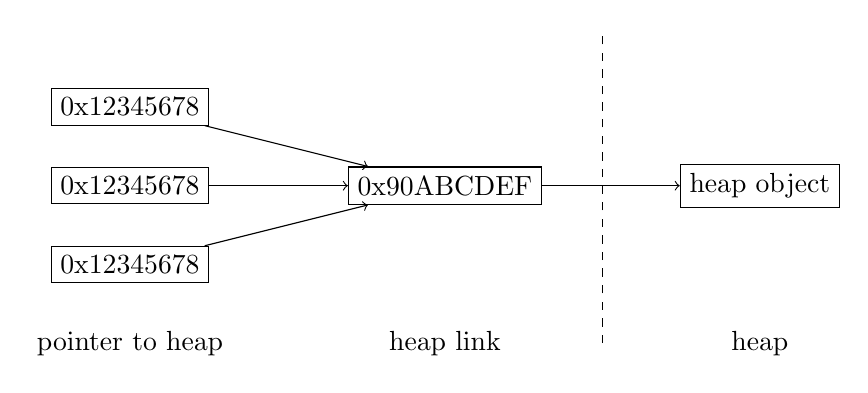
\begin{tikzpicture}
\node [rectangle, draw] (p1) at (0,1) {0x12345678};
\node [rectangle, draw] (p2) at (0,0) {0x12345678};
\node [rectangle, draw] (p3) at (0,-1) {0x12345678};
\node at (0,-2) {pointer to heap};
\node [rectangle, draw] (hl) at (4,0) {0x90ABCDEF};
\node at (4,-2) {heap link};
\node [rectangle, draw] (heap) at (8,0) {heap object};
\node at (8,-2) {heap};
\draw [->] (p1) -- (hl);
\draw [->] (p2) -- (hl);
\draw [->] (p3) -- (hl);
\draw [->] (hl) -- (heap);
\draw [dashed] (6, -2) -- (6, 2);
\end{tikzpicture}
%%}%
\cprotect\caption{Example illustrating heap links\label{heap_link}.  The objects on the far left represent user-level pointers to heaps, e.g., \verb+* heap int+.  The middle object is a heap link, which contains the address of the child heap that appears on the far right.}
\end{figure}

As illustrated in Figure~\ref{heap_link}, a user-level pointer to a heap points to an object called a heap link which in turn points to a heap.
The objects on the left side of the diagram are objects in the parent heap and the object on the right is the child heap.
The extra level of indirection introduced by the heap link concentrates all references to the child heap into one location.
Moving a heap involves reading the pointer out of the heap link and replacing it with \verb+nil+.
This makes the heap inaccessible to the previous owner (parent), which maintains the isolation of state between reactive components.
The marking phase of the mark-and-sweep algorithm is aware of heap links and marks heaps as being reachable from another heap.
Unreachable heaps are pruned from the hierarchy during garbage collection.

\paragraph{Embarrassingly parallel garbage collection.}
Two features of reactive components permit concurrent garbage collection.
First, the state of each reactive component is isolated which allows garbage collection to be performed on different components at the same time without conflict.
Second, garbage collection can be framed as an action to be executed by the scheduler.
Thus, associated with each component is an action that invokes the garbage collector on the implicit and explicit heaps of the corresponding component.
Furthermore, the action is considered to modify the state of the component which prevents all transactions involving the component from executing concurrently with the garbage collection action.
We assume that the scheduler selects the garbage collection action often enough that no additional invocations of the garbage collector are necessary.
More plainly, we do not trigger the garbage collector in the allocation routine, which is the approach taken by many systems using garbage collection.
Most garbage collection algorithms include a scan of the call stack as objects reachable from the call stack must not be collected.
In our approach, such scanning is useless since the call stack is empty when executing the garbage collection action and the root object is embedded in the implicit heap that is being collected.

\section{I/O}

A bottom-up approach which may lead to the adoption of reactive components is to write a kernel for reactive components, i.e., a scheduler and memory manager, and proceed to replace the operating system and applications.
This approach is impractical and risky given the expense of developing software for an unproven technology.
A top-down approach involves proving the utility of reactive components at the application layer and then proceeding to lower layers when appropriate.
This approach far less risky and the one taken in this chapter.
To develop and evaluate real-world applications, the input/output facilities of the host operating system must be exposed to reactive components so that they may communicate and interact with other processes and systems.
This section describes our approach to exposing the input/output (I/O) facilities of a Linux/GNU system to reactive components.

A Linux/GNU system offers a variety of I/O and communication mechanisms including pipes, sockets, shared memory, and message queues.
For our purposes, we focused on mechanisms that are available through a file descriptor interface.
Our approach consists of two steps.
The first step is to add file descriptors and operations for manipulating them, such as read and write, to the language.
The second step was to wrap file descriptors in reactive components to make their functionality available via a conventional reactive component interface.

The main consideration when supporting file descriptors was to ensure that reads and writes were non-blocking as a blocking read or write may violate weak fairness.
A transaction that blocks on a read or write would adversely affect the latency and throughput of the scheduler as the scheduler thread would be blocked and not able to service other transactions.
Furthermore, a blocking transaction holds the locks for all components involved in that transaction and other enabled transactions that also involve those components would be denied service which violates the weak fairness requirement of the scheduler.
To prevent these problems, all file descriptors when they are created are set to be non-blocking.
Thus, all subsequent reads and writes are also non-blocking.

Threaded programs using non-blocking I/O typically use some kind of synchronous I/O multiplexing which allows a thread to determine which file descriptors are ready for reading and/or writing.
The goal in doing so is to allow a thread to service multiple file descriptors and yield the processor if no file descriptors are ready.
To map this concept into reactive components, we introduced a \verb+readable+ function that tests if a file descriptor is ready for reading and a \verb+writable+ function that tests if a file descriptor is ready for writing.
These functions are intended to be used in preconditions so that an action becomes enabled when the corresponding file descriptor is ready.

The \verb+readable+ and \verb+writable+ functions are also used as part of the termination protocol.
When the termination protocol enters the checking phase where it attempts to prove that every precondition is false, it records which file descriptors are being checking for readability and writability.
If the termination protocol proves that all preconditions are false but some preconditions depend on readability or writability, it enters a state where it waits for one of the file descriptors to become ready.
This allows a system of reactive components to sleep while it waits for external input like a message from a remote host or a timer.
Currently, the Partitioned scheduler is the only scheduler that supports this behavior.

Conceptually, a file descriptor contains component state and should be subject to all of the constraints of normal component state.
The two main constraints are 1) it cannot be shared by another component and 2) it cannot change in the immutable phase of a transaction.
To enforce the first constraint, file descriptors are implemented as dynamically allocated opaque data structures.
Forcing dynamic allocation makes file descriptors subject to the pointer sharing rules, i.e., they can only be shared via foreign dereference mutability in the immutable phase.
Making the data structure opaque prevents sharing through copying.
The normal immutable phase rules in concert with properly declared builtin functions prevent file descriptors from changing in the immutable phase.
That is, functions like \verb+read+ and \verb+write+ require a pointer to a file descriptor with mutable dereference mutability.

To test these ideas, we implemented a Simple Network Time Protocol (SNTP) client.
SNTP attempts to acquire the current time from a server while simultaneously measuring a round-trip latency to determine an accurate local time.
The client timestamps the request with the local time and sends it to the server.
The server timestamps the request when it arrives and again when it sends it back to the client.
Finally, the client timestamps the request when it receives it back from server.
The client uses the timestamps to determine the offset of the local clock from the clock on the server.
This procedure is repeated periodically to resynchronize the local clock.
The messages are exchanged using the User Datagram Protocol (UDP).

\begin{figure}
\centering
\resizebox{\textwidth}{!}{%
\begin{tikzpicture}
\draw (2,7.5) rectangle (4,9);
\node[below] at (3,9) {Timer};
\rapush[4,8,1.8,.5,alarma,ignore]{Alarm()};

\draw (1.5,6) rectangle (16.5,10);
\node[below] at (8.5,10) {Sntp};
\lppush[5,8,1.8,.5,alarmb,ignore]{Alarm()};
\rapush[11,8,3.5,.5,senda,ignore]{Send(UdpMessage)};
\rppush[11,7,4.1,.5,receivea,ignore]{Receive(UdpMessage)};

\draw (12,6.5) rectangle (16,9);
\node[below] at (14,9) {UdpParticipant};
\lppush[12,8,3.7,.5,sendb,ignore]{Send(UdpMessage)};
\lapush[12,7,3.8,.5,receiveb,ignore]{Receive(UdpMessage)};

\draw (alarma.center) -- (alarmb.center);
\draw (senda.center) -- (sendb.center);
\draw (receivea.center) -- (receiveb.center);

\end{tikzpicture}
}%
\caption{Diagram of a Simple Network Time Protocol (SNTP) client\label{sntp}}
\end{figure}

Figure~\ref{sntp} shows a diagram of the SNTP client application.
The top-level Sntp component contains two sub-components:  Timer and UdpParticipant.
The Timer component is a periodic timer implemented by wrapping a ``timerfd'' file descriptor.
The UdpParticipant component wraps a UDP socket file descriptor and is capable of sending and receiving UDP messages.
The Sntp component uses these components to implement an SNTP client.
Whenever the Timer fires the alarm, the UdpParticipant creates an SNTP request and sends it using the UdpParticipant.
This all happens as part of one atomic transaction.
Whenever the UdpParticipant receives a message, it passes it to the Sntp component which deserializes it, timestamps it, and interprets it to compute the local clock offset.

The Sntp component demonstrates how composition can be used to construct systems.
The Timer and UdpParticipant components are generic since they do not contain any SNTP related logic.
Furthermore, they have well-defined concurrency semantics that will be enforced when they are composed in other systems.
Thus, it is possible to use the reactive component model to produce reusable \emph{reactive} software.

\section{Scheduler}
\label{scheduler}

A scheduler is responsible for selecting and executing transactions according to the weak fairness criteria set forth in Chapter~\ref{model}.
Of particular interest is the design and implementation of general-purpose schedulers that are capable of executing transactions in parallel.
The main inputs to a scheduler are the transactions enumerated by the composition analysis.
The access sets calculated for each transaction are used by concurrent schedulers to avoid non-deterministic state transitions.
We introduce some of the issues involved in designing and implementing a scheduler for reactive components, through a series of increasingly complex scheduler designs.
The two concrete implementations described later will draw upon the designs of these schedulers.

\subsection{The Scheduling Problem}
\label{scheduling_problem}

A scheduler is responsible for mapping transactions to processor cores so that they can be executed according to the semantics of reactive components.
As described in Chapter~\ref{model}, concurrent execution is modeled by a scheduler that serially and repeatedly selects and executes atomic transactions according to weak fairness, which means that an enabled transaction must eventually be selected and executed.
A scheduler implementation supporting concurrent execution must take care to preserve the fairness and atomicity required by the model.
A scheduler is \emph{fair} if it meets the weak-fairness criteria set forth in Chapter~\ref{model}.
A scheduler is \emph{safe} if it avoids conditions where one transaction is changing the state of a component while another transaction is reading or writing the same state.
The execution of a transaction in a safe scheduler is logically atomic.

A scheduler is \emph{responsible} if it only terminates when the precondition for every transaction is false.
Such a state is called a \emph{fixed point}.
A scheduler may terminate responsibly when the system reaches a fixed point because no action will be selected and executed meaning that no component will change state.
Termination is not a requirement for a scheduler but it is useful from the perspective of testing and evaluation.
We are interested in designing fair, safe, and responsible schedulers, as these schedulers enforce the semantics of reactive components.

We model a scheduler as a state transition system consisting of a set of possible states $S$, an initial state $s_0 \in S$, and a transition function $\sigma: S \to S$.
The function $\sigma$ is applied to the current scheduler state $s$ to generate the next scheduler state $s' = \sigma (s)$.
To refer to previous scheduler states, we assign a logical time $t \in \mathcal{N}$ to each scheduler state so that $s(t + 1) = \sigma (s(t))$.
Using this notation, the initial state of the scheduler is $s(0) = s_0$.
The definitions of $S$, $s_0$, and $\sigma$ will be unique to each scheduling algorithm.
We are interested in the properties of $\sigma$ as they relate to enforcing the scheduling semantics of reactive components and how these properties help or hinder a scheduler implementation.

The generic state of a scheduler is modeled as a vector where each element of the vector contains the scheduling state associated with a particular transaction.
Let $s \in S$ be a generic scheduler state and let $T$ be the set of transactions.
The value $s_u(t)$ represents the scheduler state for transaction $u \in T$ at time $t$.
Each value $s_u(t)$ is a pair $(p, q)$.
The value $p \in \{\bot, 0, 1\}$ represents the precondition of the transaction known by the scheduler as either unknown ($\bot$), false (0), or true (1).
The value $q \in Q = \{\mathit{Idle}, \mathit{Eval}, \mathit{Exec}\}$ represents the state of the transaction as either being idle, evaluating the precondition, or executing the immutable and mutable phases.
Initially, all transactions start with an unknown precondition in the idle state:
\begin{equation}
  \forall u \in T : s_u(0) = (\bot, \mathit{Idle})
\end{equation}

In the model, the precondition of each transaction is always defined and known since the state against which the preconditions are evaluated is always defined and known due to atomicity.
In a real scheduler, the execution of a transaction takes time and the state of all involved components is not defined for this duration.
Consequently, the values of preconditions derived from this state are also not defined during the same duration.
After a transaction, all preconditions based on any mutated state are undefined and must be re-evaluated to determine if they are true or false.

\begin{figure}
\centering
%\resizebox{\textwidth}{!}{%
\begin{tikzpicture}
  [->,-triangle 60, node distance=3cm, auto, every loop/.append style={-triangle 60}]

  \node[initial,state] (I)              {$I$};
  \node[state]         (V) [above of=I] {$V$};
  \node[state]         (X) [right of=I] {$X$};

  \path (I) edge [bend left] node {$a$} (V)
            edge [bend left] node {$e$} (X)
        (V) edge [bend left] node {$d$} (I)
            edge             node {$b$} (X)
        (X) edge [bend left] node {$c$} (I);

  \path (I) edge [loop below] node {$\lambda$} ();
  \path (V) edge [loop above] node {$\lambda$} ();
  \path (X) edge [loop right] node {$\lambda$} ();

\end{tikzpicture}
%}%
\caption{State transition diagram for the state component of dynamic transaction state.
  $I$ represents $\mathit{Idle}$, $V$ represents $\mathit{Eval}$, and $X$ represents $\mathit{Exec}$.
  \label{dt_state}}
\end{figure}

The dynamic transaction state $s_u(t)$ is itself a state transition system and much of the challenge in designing a scheduler revolves around the details of enforcing this transition system for concurrently executing transactions.
Figure~\ref{dt_state} shows the state transition diagram for the state component of dynamic transaction state ($q$ of $s_u(t)$).
Each state has a self loop that allows a transaction to stay in the same state while another transaction changes state (indicated by $\lambda$).
There are two main paths through the transition system.
The path $abc$ corresponds to evaluating the precondition and immediately executing the immutable and mutable phases.
The path $adec$, for example, corresponds to evaluating the precondition and later executing the immutable and mutable phases.
Let $\Gamma$ be the set of transitions indicated in Figure~\ref{dt_state}.
Each element $\gamma \in \Gamma$ is a pair in $Q \times Q$.
The following condition states that every transition in a scheduler must obey the transition system described in Figure~\ref{dt_state}:
\begin{equation}
  \forall t, u : (s_u(t).q, s_u(t+1).q) \in \Gamma
\end{equation}
The precondition of a transaction is established as true or false as a result of leaving the $\mathit{Eval}$ state (transitions $b$ and $d$ in figure~\ref{dt_state}):
\begin{equation}
  \label{pre_establish}
  \forall t, u, s_u(t).q = \mathit{Eval} \land s_u(t+1).q \neq \mathit{Eval} : s_u(t+1).p \in \{0,1\}
\end{equation}
The precondition of a transaction must be true while executing the immutable and mutable phases:
\begin{equation}
  \label{pre_true}
  \forall t, u : s_u(t).q = \mathit{Exec} \implies s_u(t).p = 1
\end{equation}

A transaction that mutates the state of one or more components invalidates the precondition of all transactions whose preconditions are derived from the same state.
Let $\mathit{pre}: T \to H$ be a function that maps a transaction to the set of access pairs corresponding to the precondition of a transaction.
Let $\mathit{imm}(u)$ and $\mathit{mut}(u)$ be similarly defined functions that return the immutable phase access set and mutable phase access set for transaction $u \in T$.
All of these functions may be computed as part of composition analysis.
The set of transactions that are potentially affected by a given transaction $u \in T$ is given by the following function:
\begin{equation}
  \label{affected}
  \mathit{affected}(u) = { v \in T : \mathit{race}(\mathit{mut}(u), \mathit{pre}(v)) }
\end{equation}
The result of a transaction being executed has the effect of invalidating the precondition for all affected transactions:
\begin{multline}
  \forall t, u : s_u(t).q = \mathit{Exec} \land s_u(t+1).q \neq \mathit{Exec} \implies \\ \forall v \in \mathit{affected}(u) : s_v(t+1).p = \bot
\end{multline}
The previous requirement represents a worst case scenario where the transaction mutates all components in the mutable access set.
An obvious optimization is to only invalidate preconditions derived from the subset of instances that actually changed state.

A scheduler is safe if it avoids data races among the set of active transactions.
We define the dynamic access set of a transaction as follows:
\begin{equation}
  \label{access}
  \mathit{access}(s_u) = \begin{cases}
    \emptyset & \text{if $s_u.q = \mathit{Idle}$} \\
    \mathit{pre}(u) & \text{if $s_u.q = \mathit{Eval}$} \\
    \mathit{imm}(u) \cup \mathit{mut}(u) & \text{if $s_u.q = \mathit{Exec}$}
    \end{cases}
\end{equation}
A scheduler state is safe if there are no data races:
\begin{equation}
  \mathit{safe}(s) = \forall u, v \in T, u \neq v : \lnot \mathit{race} (\mathit{access}(s_u), \mathit{access}(s_v))
\end{equation}
A scheduler is safe if it only enters safe states:
\begin{equation}
  \label{race}
  \forall t : \mathit{safe}(s(t))
\end{equation}

%% The safety requirement expressed in equation~\ref{race} influences every voluntary scheduling decision.
%% Consider the set of possible next states for a scheduler.
%% The transitions in figure~\ref{dt_state} can be classified into two groups.
%% Transitions $a$, $b$, and $e$ are voluntary and result in non-empty access sets while $d$ and $c$ are involuntary and result in empty access sets (equation~\ref{access}).
%% Thus, we limit the discussion to scheduling steps where the scheduler is making a voluntary transition.
%% Let $\mathit{vol}(t) \subseteq T$ represent the subset of transactions that are candidates for a voluntary transition at time $t$ and let $\mathit{next}(u)$ represent the next transition state according to the system of figure~\ref{dt_state}.
%% Also, let $s(t) \downarrow u$ represent the result of substituting transaction state $u$ into $s(t)$.
%% A set of possible next states is given by:
%% \begin{equation}
%%   \mathit{candidates}(t) = \bigcup_{u \in \mathit{vol}(t)} s(t) \downarrow \mathit{next}(u)
%% \end{equation}
%% However, not every state in $\mathit{next}(t)$ is a valid state due to equation~\ref{race}.
%% A refined set of next states is then:
%% \begin{equation}
%%   \mathit{next}(t) = \{ s \in candidates(t) : safe(s) \}
%% \end{equation}

In a weakly fair scheduler, an enabled transaction cannot be postponed indefinitely.
Argument by contradiction is one approach to demonstrating that a scheduling algorithm is weakly fair.
If one assumes that a scheduler is not weakly fair, then there must be some scheduler state $s(t_c)$ that contains a transaction $u$ that is enabled in every subsequent state but never executed.
The ``enabledness'' described in the previous sentence is not the value $p$ in the definition of $s_u(t)$ which is the value known by the scheduler.
Rather, it refers to the actual value of the precondition based on the state contained in the component instance.
The argument is completed by demonstrating that the scheduler does in fact execute $u$.
For example, a scheduler that processes transactions in last-in first-out (LIFO) order eventually selects and executes every transaction in the queue.

A scheduler design must reconcile the forces arising from the basic execution model, fairness, and safety.
The basic execution model forces the scheduler to establish preconditions (Equation~\ref{pre_establish}) before executing the immutable and mutable phases (Equation~\ref{pre_true}).
Weak fairness compels the scheduler to select and execute certain transactions while safety compels the scheduler to avoid selecting and executing certain transactions (equation~\ref{race}).
To illustrate the interplay between these two forces, consider a concurrent, and work-conserving scheduler.
Suppose that all transactions in the system are safe with respect to each other save one designated $\tau$ and that $\tau$ is not active.
Since the scheduler is work-conserving, it will continue to select transactions but continue to avoid selecting $\tau$ for safety.
Thus, with respect to parallel execution, a scheduler may be forced to sacrifice some parallelism to ensure fairness.

The scheduling problem for reactive components, then, is:  given a set of active transactions, select the next transaction for evaluation (precondition) or execution (immutable and mutable phase) subject to weak fairness and safety.

\subsection{Scheduler Classes}

\paragraph{Lazy and eager schedulers.}
A scheduler may be \emph{lazy} or \emph{eager} with respect to evaluating preconditions.
A lazy scheduler defers evaluating the precondition until the transaction is selected for execution (path $abc$ in Figure~\ref{dt_state}).
An eager scheduler evaluates preconditions after the state upon which they are based changes (path $ad$ in Figure~\ref{dt_state}).
The perceived benefit of a lazy scheduler is that it may reduce overhead by not evaluating preconditions while the perceived benefit of an eager scheduler is that it may only select actions which are enabled which may result in more efficient use of acquired resources.

\paragraph{Oblivious and knowledgeable schedulers.}
We have considered two kinds of schedulers with respect to safety.
The first is an \emph{oblivious} scheduler that doesn't have direct access to the (global) scheduler state and therefore can't know the set of next states.
An oblivious scheduler selects a transaction and then determines if the transaction is safe to execute.
This typically involves a locking mechanism to ensure that all of the instances in the requisite access sets are available.
The second kind of scheduler is a \emph{knowledgeable} scheduler that does know the global scheduler state.
A knowledgeable scheduler can be proactive and maintain a set of transactions that are safe with respect to the set of active transactions.
This would allow a knowledgeable scheduler to efficiently select a safe action.
The open question is whether or not the efficiency of selection overcomes the overhead of maintaining the set of safe transactions.

\paragraph{Cautious and speculative schedulers.}
A \emph{cautious} scheduler avoids all race conditions and always satisfies the safety requirement of Equation~\ref{race}.
A \emph{speculative} scheduler optimistically evaluates preconditions and executes transactions and aborts them if a conflict is discovered.
Transactional memory is one technology that could be used to build a speculative scheduler.
For this work, we will assume that preconditions, immutable phases, and mutable phases are not aborted and leave the application of transactional memory to reactive components as future work.

\paragraph{Non-preemptive and preemptive schedulers.}
An \emph{active} transaction is one whose precondition is being evaluated or whose immutable or mutable phase is being executed.
An active transaction need not physically occupy a processor core.
This condition occurs in \emph{preemptive} schedulers that can interrupt a precondition, immutable phase, or mutable phase to do other work.
In contrast, a \emph{non-preemptive} scheduler does not interrupt the execution of a transaction, i.e., transactions are physically atomic.
Preemption may be useful to reduce the latency of transactions, support real-time priorities, etc.
We leave the application of preemption to reactive component schedulers as future work.

\subsection{Scheduler Design}

The previous sub-section illustrated a number of design dimensions for reactive component schedulers:  lazy vs. eager, oblivious vs. knowledgeable, cautious vs. speculative, and non-preemptive vs. preemptive.
For tractability, we will focus on the design and implementation of particular schedulers that are lazy, oblivious, cautious, and non-preemptive, and leave a more complete exploration of the design space for future work.
The goal of the following discussion is to introduce some of the issues when designing and implementing a scheduler through a series of increasingly complex scheduler designs.
We will describe the concurrent schedulers in terms of \emph{threads}, which may correspond to physical processor cores or threads in an operating system.

%% \paragraph{Scheduler criteria.}
%% A scheduler is \emph{fair} if it meets the weak-fairness criteria set forth in chapter~\ref{model}.
%% A scheduler is \emph{safe} if it avoids conditions where one transaction is changing the state of the component while another transaction is reading or writing the same state.
%% A scheduler is \emph{responsible} if it only terminates when the precondition for every action is false.
%% Obviously, we are interested in fair, safe, and responsible schedulers as these schedulers enforce the semantics of reactive components.
%% The final criteria for a scheduler is efficiency which typically refers to either the computational complexity or storage complexity associated with its operation.
%% % Of primary interest is the \emph{selection efficiency} or the amount of computation required for the scheduler to determine the next action to execute.

\paragraph{Serial round-robin scheduler.}
Perhaps the simplest scheduler that can be implemented is a serial round-robin scheduler.
This design may be appropriate in the context of uniprocessor embedded systems with tight resource constraints.
The scheduler repeatedly cycles through the list of transactions, evaluating the precondition of each transaction and executing the immutable and mutable phases if the precondition was true.
If no transaction is executed in a cycle, then the scheduler terminates.
This scheduling algorithm is fair by virtue of the strict round-robin policy, safe from the fact that it is serial and non-preemptive, and responsible by definition.
The \emph{selection efficiency} of a scheduler is the number of transactions that must be selected before executing a transaction or terminating.
The selection efficiency of this algorithm is $O(|T|)$ as illustrated by a system where one transaction that is perpetually enabled while all of the other transactions are perpetually disabled.

\paragraph{Serial scheduler with a transaction work queue.}
The perceived weakness of the serial round-robin scheduler is the overhead of evaluating preconditions that evaluate to false.
So, instead of cycling through the list of transactions, this scheduler maintains a work queue of transactions whose preconditions are true.
At initialization time, the scheduler populates the queue by evaluating the precondition for all transactions in the system.
The scheduler then repeatedly takes a transaction from the queue, executes it, and then inserts any newly enabled transactions, making this scheduler an eager scheduler.
To find newly enabled transactions, the scheduler uses the access set generated during composition analysis.
That is, after executing a transaction, the scheduler tests all of the transactions for the components in the access set and adds them to the queue if necessary.
Alternatively, the scheduler may assume that the precondition is true and insert the transaction knowing that the precondition will be re-evaluated when the transaction is selected.
The scheduler terminates when the work queue is empty.
This scheduling algorithm is fair if the work queue is processed in first-in first-out (FIFO) order, safe because the algorithm is serial and non-preemptive, and responsible since an empty work queue implies no transaction is enabled.

The pathological scenario for the serial round-robin scheduler applies to this scheduler as well, so the worst-case selection efficiency of the algorithm is $O(|T|)$.
Assume that the most complex transaction in the system involves $c$ components and some component has a system maximum transaction count of $a$.
In the worst case, the scheduler must evaluate $c \times a$ preconditions for every transaction that it executes.
Thus, the overhead associated with this scheduler is related to the compositional structure of the system that it is executing.
This overhead may be acceptable for systems where $c$ and $a$ are small or for systems whose average work queue size is small compared to the total number of transactions in the system.
This suggests that the average number of enabled transactions compared to the total number of transactions may be a useful way to analyze reactive component systems and schedulers.
For example, the serial round-robin scheduler would be appropriate for a \emph{heavily enabled} system while the serial scheduler with a transaction work queue would be appropriate for a \emph{lightly enabled} system.

\paragraph{Serial scheduler with an instance work queue.}
This scheduling algorithm attempts to squeeze a little more performance from the single-threaded scheduler with a transaction work queue.
The significant difference is that after the scheduler executes a transaction, it places the component instances that might have changed state into the work queue.
The work queue is initialized with all of the components in the system.
When processing a component on the work queue, the scheduler cycles through all of the transactions for that particular component.
The potential increase in performance comes from deferring the evaluations of the preconditions until absolutely necessary, i.e., lazy scheduling.
The scenario on which this scheduler attempts to capitalize is when some components are rarely involved in transactions.
An instance is enabled if at least one of its transactions is enabled.
Thus, this scheduler is appropriate for systems that are lightly enabled from the instance perspective.

\paragraph{Concurrent global round-robin scheduler.}
This scheduler runs $P > 1$ copies of a round-robin scheduler in parallel.
To be safe, we must devise a protocol that allows the threads to avoid concurrently executing transactions that may mutate the same state.
Using the assumption that a component instance is a proxy for its state variables, the scheduler locks all instances in the access set before evaluating the precondition and executing the transaction.
Recall that composition analysis determines the set of components that are involved in a transaction and how they are accessed ($\mathit{Read}$ or $\mathit{Write}$).
The acquired lock corresponds to the access type, which allows multiple threads to be reading a component but only one thread to be writing.
The locks are acquired in a determined order to avoid deadlock (Havender's Principle).
The concurrent global round-robin scheduler is fair so long as the underlying locking mechanism is fair, i.e., there is no reader or writer starvation.
The algorithm is also responsible as each thread proves to itself that there are no enabled transactions left in the system.

An important concern with this algorithm is the locking required to coordinate access to component instances.
One negative characteristic caused by the locking is that a thread may become idle while waiting for a lock.
Thus, we might look for alternatives that allow a thread to do useful work while waiting for a lock.
Another goal might be to look for ways to coordinate access to component instances without using locks at all.
Some of these ideas are explored later in this chapter.

\paragraph{Concurrent partitioned round-robin scheduler.}
Rather than have each thread cycle through the entire list of transactions, the concurrent partitioned round-robin scheduler divides the list of transactions among the available threads.
Like the global version, this algorithm is fair if the underlying locking mechanism is fair.
Similarly, this algorithm is safe as locks are used to coordinate access to component state.
However, for this algorithm to be responsible, we must add a protocol that allows the threads to detect that the system has reached the termination condition.

The termination protocol consists of a barrier synchronization and then a check to establish the termination condition.
The termination protocol begins when a scheduler thread sends a termination request to the \emph{manager thread}.
To process a termination request, the manager thread stops each scheduler thread and then checks that all transactions are disabled.
If all of the transactions are disabled, the system terminates.
Otherwise, the manager thread restarts the scheduler threads.
A scheduler thread may choose to request termination at any time and different heuristics may be used to determine when a scheduler thread makes the termination request.
Deferring the request has the advantage of avoiding the termination protocol overhead.
For example, a scheduler thread might wait until it makes a complete pass through its list of transactions without executing one before making the request.

Such a centralized termination protocol is rather disruptive as it must stop the system to check for termination.
Thus, one goal may be to let a thread idle itself and be woken up by active neighbors.
Similarly, the scheduler threads can check for the termination condition in parallel and wake up all of their neighbors if a transaction is enabled.
Finally, the manager thread may be done away with entirely and the protocol rewritten as a distributed protocol, as we discuss below.

\subsection{Scheduler Implementation}

\paragraph{Concurrent scheduler with a global instance work queue.}
The first scheduler that we implemented was a concurrent scheduler with a global instance work queue.
The work queue is initialized to contain all of the instances in the system.
The scheduler threads take an instance from the work queue, select and execute all transactions in the instance, and insert any instances that might have changed state back into the work queue.
Fairness is achieved by processing the queue in LIFO order and safety is achieved through the aforementioned locking scheme.
The termination protocol for this scheduler involves counting the number of instances that are currently in the queue and the number of instances currently being processed by the scheduler threads.
When this count drops to zero, there are no enabled instances in the system and the system may terminate responsibly.

One potential weakness of this scheduler is the synchronization required to coordinate access to the work queue, which adds a communication overhead and may create contention if the scheduler threads are lightly loaded, i.e., they frequently return to the queue looking for work.
Thus, the scalability of this scheduler is a concern.

\paragraph{Concurrent partitioned round-robin scheduler with asynchronous locking and distributed termination.}
One of the goals when designing this scheduler was to avoid the blocking behavior and overhead of locking observed with the concurrent scheduler with a global instance work queue.
The reader/writer locks used to protect each component instance were replaced by asynchronous read/writer locks implemented in user-space.
The asynchronous locks consist of a spin lock, variables indicating the status of the lock, and a queue of requests.
To acquire a lock for a component, a scheduler thread first acquires the spin lock and then checks if the lock can be acquired immediately, which it can if either the lock has no owner or the thread is a reader (i.e., it is requesting a read lock); the lock has already been locked by another reader; and there are no writers in the queue.
Otherwise, the request is placed on the queue.
A scheduler thread failing to acquire the lock can either idle or attempt to execute a different transaction.
When a lock is unlocked, the thread at the front of the queue is notified so it may resume processing the transaction that it was attempting to execute.
The protocol avoids reader and writer starvation and ensures fairness since the queue is processed in LIFO order.
This scheduler is \emph{work conserving} since a scheduler thread continues to execute transactions instead of blocking.
However, scheduler threads do not steal work from other threads.

The aforementioned centralized termination protocol has the potential to be disruptive.
Thus, the motivation for a distributed termination protocol is to keep the scheduler threads as busy as possible meaning that the termination protocol is started infrequently and the termination protocol itself aborts as early as possible if the termination condition has not been reached.
For this scheduler, the threads are arranged in a ring and communicate using asynchronous message queues.
Messages are stamped with the id of the originating thread.
Some parts of the protocol forward messages around the ring so a thread receiving a message from itself knows that all of the threads have processed that message.

Like the centralized version, the ring-based distributed termination protocol consists of a synchronization phase and checking phase.
Scheduler threads begin in the RUN state where they are actively cycling through their lists of transactions.
When a scheduler thread determines that termination may be possible, it sends a message to its neighbor indicating that it is entering the SYNC state.
If the neighbor thread is in the RUN state, it resolves to send a reset message the next time it executes a transaction which means that the termination condition has not been established.
Otherwise, the neighbor thread itself is already in the SYNC state and forwards the message.
Reset messages are unconditionally forwarded around the ring and cause all threads to enter the RUN state.
Synchronization messages are only forwarded if the thread receiving the message is in the SYNC state.
Thus, if a thread receives its own synchronization message, all other threads in the scheduler are in the SYNC state.
Multiple threads may receive their own synchronization message at the same time.

The goal of the synchronization phase is to establish a common point of reference for determining if any transaction is enabled.
When a thread receives its own synchronization message, it sends a message to its neighbor that it is entering the CHECK state.
This message is forwarded around the ring causing all of the threads to enter the CHECK state.
The CHECK state is like the modified RUN state in that any executed transaction causes a reset message to circulate around the ring.
A thread that cycles through its list of transactions and finds no enabled transactions sends a wait message to its neighbor and enters the WAIT state.
If the neighbor is in the WAIT state, it forwards the message.
If a thread receives its own wait message, then all of the threads are in the WAIT state and the termination condition has been established.
Upon receiving its own wait message, a thread sends a termination message causing all threads to terminate.

\subsection{Scheduler Evaluation}

The utility of the reactive component model rests on the ability to execute reactive programs effectively.
The challenge, then, is to design and implement effective schedulers subject to the constraints and limitations imposed by the model.
The exercise of developing and evaluating schedulers may suggest possible improvements to the model or provide evidence that core features of the model resist efficient implementation.
The definition of an effective scheduler will vary by platform and problem domain.
For example, embedded systems may prefer a single-threaded scheduler with minimal memory requirements and power-awareness.
Our focus in this work is to make progress on a general purpose concurrent schedulers.

We propose the following metrics for the evaluation of a general-purpose scheduler:
\begin{description}
\item[Throughput:] the number of transactions executed per second.
Given the same system, a scheduler with higher throughput is preferable to a system with lower throughput as it is accomplishing more work per unit of time.
Throughput can also be defined for specific problems by defining a unit of work and measuring the number of work units processed per unit of time.
\item[Latency:] the amount of time between an transaction becoming enabled and being executed.
The goal in measuring the latency between a transaction becoming enabled and its execution is to quantify the responsiveness of the scheduler.
An interactive application may prefer a scheduler that executes enabled transactions promptly to aid in providing a good user experience or other benefit.
Like throughput, latency may also be defined for units of work.
\item[Utilization:] the fraction of the CPU used.
Utilization is a measure of how efficiently the scheduler is using the CPUs and can be used to quantify an improvement in throughput or latency.
For example, a 10\% increase in throughput accompanied by a 10\% increase in utilization may be acceptable while a 10\% increase in throughput with a 100\% increase in utilization may not be acceptable.
\end{description}
Both throughput and latency may be considered for individual transactions or aggregated over all transactions in the system.

\paragraph{Evaluation approach.}
We used two variants of the clock system from Chapter~\ref{model} to evaluate the two scheduler implementations.
The first variant is the fully-factored clock system augmented with counters that cause termination\footnote{https://github.com/jrw972/rc/blob/master/samples/clock3.rc}.
In this system, there are three components of interest:  the Client, the Server, and the Counter.
This system has three transactions:
\begin{itemize}
  \item Request - The client requests the time from the server.  This involves the Client and the Server.
  \item Response - The server responds with the time.  This involves the Client, the Server, and the Counter.
  \item Tick - The counter increments the current time.  This involves the Counter.
\end{itemize}
This system will be denoted as the \emph{AsyncClock} system.

\begin{figure}
\centering
\resizebox{.5\textwidth}{!}{%
\begin{tikzpicture}

\node[draw, ellipse] (Request) at (0,0) {Request};
\node[draw, ellipse] (Response) at (3,0) {Response};
\node[draw, ellipse] (Tick) at (1.5,-1) {Tick};

\draw (Request) -- (Response);
\draw (Tick) -- (Response);

\end{tikzpicture}
}%
\caption{Race graph for the AsyncClock system.  Each node is a transaction.  Nodes sharing an edge cannot be executed concurrently due to potentially mutated shared state. \label{clock_system_mutex}}
\end{figure}

Figure~\ref{clock_system_mutex} shows a \emph{race graph} for the AsyncClock system.
Each node in the graph is a transaction $u \in T$.
Let $\mathit{acc}(u) = \mathit{pre}(u) \cup \mathit{imm}(u) \cup \mathit{mut}(u)$.
An edges exists between two nodes $u,v \in T$ if $\mathit{race}(\mathit{acc}(u), \mathit{acc}(v))$.
Nodes sharing an edge cannot be executed concurrently due to potentially mutated shared state.
Conversely, nodes that are not linked by an edge can be executed concurrently.
For the purpose of evaluating schedulers, the clock system has the important characteristic that Request and Tick can be executed concurrently while Response must be executed independently.
Another useful feature of this system is that each component has exactly one transaction, and thus, a  work queue of instances may also be viewed as a work queue of transactions.

The second variant is a simplified version of the clock system consisting of a Tick transaction that increments the counter and a Request transaction that uses a getter to sample the counter\footnote{https://github.com/jrw972/rc/blob/master/samples/clock4.rc}.
The counter creates a race between the two transactions so that they cannot be executed concurrently.
This system will be denoted as the \emph{SyncClock} system.

For comparison, we implemented threaded versions of the AsyncClock and SyncClock systems using the POSIX threads library (pthreads).
The AsyncClock implementation attempts to preserve the spirit of the AsyncClock system by being as asynchronous as possible.
This implementation uses three threads corresponding to the Request, Response, and Tick transactions.
The Request and Response threads share a flag variable that is protected by a mutex and condition variable, to implement the asynchronous request/response protocol.
The Response and Tick threads share a counter variable that is protected by a mutex.
The SyncClock implementation attempts to preserve the spirit of the SyncClock system.
In this design, there is one thread sampling the counter while another thread is incrementing the counter.
The two threads synchronize access to the counter through a single mutex.
For convenience, experiments involving a pthreads implementation will be labeled \emph{Thread}, experiments involving the concurrent scheduler with a global instance work queue will be labeled \emph{Instance}, and experiments involving the concurrent partitioned  round-robin scheduler with asynchronous locking and distributed termination will be labeled \emph{Partitioned}.

The AsyncClock and SyncClock systems were executed 1,000 times to profile the performance of each scheduler.
The programs are instrumented with profiling code that records the total execution time and timestamps for each transaction.
The timestamps are stored in memory and written after the scheduler terminates to avoid disruptions in timing due to output.
The Request and Tick transactions were limited to 10,000 executions.
Thus, each SyncClock run generates 20,000 data points.
In the AsyncClock system, the relationship between Request and Response causes Response to be executed 10,000 times as well.
Thus, each AsyncClock run generates 30,000 data points.
The throughput for a single run is determined by dividing the total number of transactions (20,000 or 30,000) by the total time used for execution.
The utilization was determined using the \verb+time+ utility and the number of context switches was determined using the \verb+getrusage+ system call before and after the execution of the system.
The latency for each transaction is determined by computing the difference between the transaction start time and the end time of the enabling transaction.
For the SyncClock system, this is $Request_{t+1} - Request_{t}$ and $Tick_{t+1} - Tick_{t}$.
For the AsyncClock system, this is $Request_{t+1} - Response_{t}$, $Response_{t+1} - Request_{t}$, and $Tick_{t+1} - Tick_{t}$.
For the SyncClock system, $1,000 \times 20,000 = 20,000,000$ latency points were collected.
For the AsyncClock system, $1,000 \times 30,000 = 30,000,000$ latency points were collected.

Placing all transactions in a run on a timeline according to their start times, we define the \emph{entanglement} of a run to be the number of adjacent transactions on the timeline that were executed in different threads.
The entanglement is used to measure the granularity of the concurrency between the scheduler threads.
Given that each run executes the same number of transactions, a high entanglement indicates ``fine'' concurrency, i.e., threads are executing transactions in parallel or execution is rapidly alternating between the threads, while a low entanglement indicates ``coarse'' concurrency.
Entanglement may be forced by the scheduler, or may occur opportunistically, or not at all.
The start time for threads influences entanglement as an operating system may execute a thread to completion before starting another thread.
The garbage collection actions are not included in the entanglement calculation to facilitate comparison with the pthread implementations.

\begin{table}
\center
\begin{tabular}{rl}
Machine Model:    & Lenovo G570 Laptop \\
Operating System: & Ubuntu 14.04 \\
Processor:        & Intel Pentium B960 2.20GHz \\
Architecture:     & 64-bit \\
Cores:            & 2 \\
Memory:           & 4GB \\
Kernel:           & 3.13.0-77-generic \#121-Ubuntu SMP \\
Compiler:         & g++ 4.8.4 \\
C library:        & glibc 2.19 \\
POSIX threads:    & glibc 2.19 \\
C++ library:      & glibc++ 3.4.19 \\
\end{tabular}
\caption{Experimental environment used for scheduler testing.\label{environment}}
\end{table}

Table~\ref{environment} describes the environment used to perform the scheduler experiments\footnote{The version of the code used for this evaluation bears the tag ``clock\_experiment2'' and can be found at https://github.com/jrw972/rc/releases/tag/clock\_experiment2.}.
The timestamp resolution reported by the operating system was 1 ns.
The Instance and Partitioned schedulers were configured to use two threads.
The Thread applications for the AsyncClock and SyncClock systems were designed to use three and two threads, respectively.
The raw data for the experiments can be obtained by emailing the author\footnote{jrw972@gmail.com}.

\paragraph{AsyncClock results.}
Figures~\ref{async_thread_throughput}, \ref{async_instance_throughput}, and \ref{async_partitioned_throughput} show histograms of the throughput for Thread, Instance, and Partitioned, respectively.
The throughput for Thread and Instance appear to have ``regular'' distributions while the throughput for Partitioned is ``irregular.''
Transactions are randomly and statically allocated to execution threads in the Partitioned scheduler.
In the AsyncClock system, there are seven transactions where three correspond to Request, Response, and Tick, and the other four correspond to garbage collection actions for Client, Server, Counter, and System components.
Thus, there are $2^7 = 128$ equally likely mappings of transactions to execution threads.
Given the symmetry of threads, this results in 64 possible arrangements which are shown in table~\ref{async_partitions}.
Some of these arrangements will place all transactions on one thread leading to improved or degraded performance, e.g., `A'.
Some arrangements will place Request and Tick on different threads allowing the potential concurrency among these actions to be exploited, e.g., `B'.
Some arrangements will place the Tick transaction and garbage collection action for Counter on different threads creating lock contention, e.g., `C'.
Thus, the throughput for the Paritioned scheduler is a mixture of distributions corresponding to the different partitioning schemes.

\begin{figure}
\center
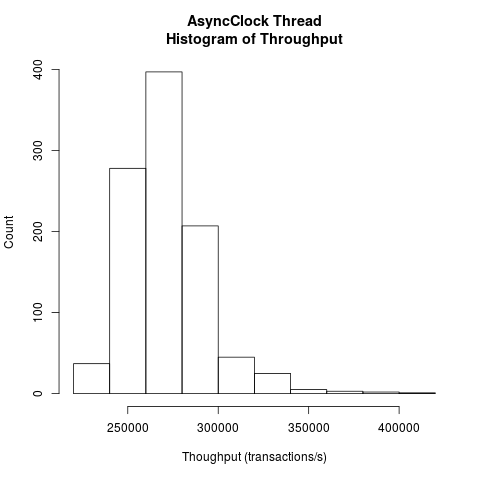
\includegraphics[height=.4\textheight]{async_thread_throughput_hist.png}
\caption{\label{async_thread_throughput}}
\end{figure}

\begin{figure}
\center
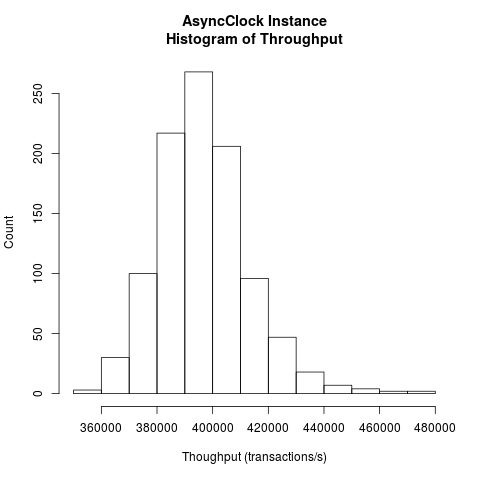
\includegraphics[height=.4\textheight]{async_instance_throughput_hist.png}
\caption{\label{async_instance_throughput}}
\end{figure}

\begin{figure}
\center
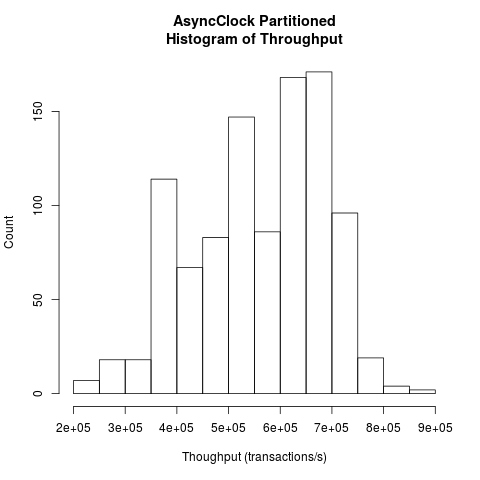
\includegraphics[height=.4\textheight]{async_partitioned_throughput_hist.png}
\caption{\label{async_partitioned_throughput}}
\end{figure}

Figures~\ref{async_thread_throughput_utilization}, \ref{async_instance_throughput_utilization}, and \ref{async_partitioned_throughput_utilization} show plots of utilization versus throughput for Thread, Instance, and Partitioned, respectively.
Most of the runs achieve a utilization greater than 100\%.
For the Instance and Partitioned schedulers, there appears to be slight trend where utilization decreases with increased throughput.
This is most likely the result of locking behavior where runs that (randomly) experience better locking behavior simultaneously achieve higher throughput and lower utilization due to less locking overhead.

\begin{figure}
\center
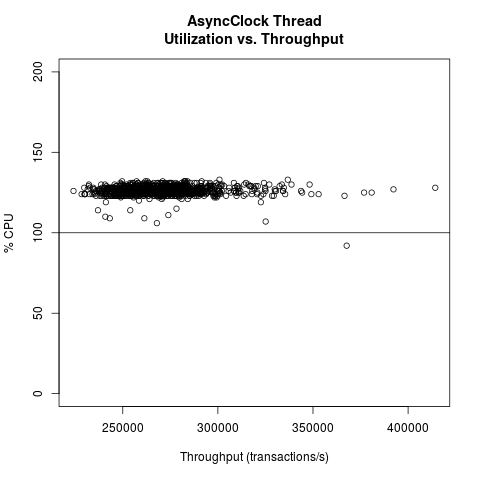
\includegraphics[height=.4\textheight]{async_thread_throughput_utilization.png}
\caption{\label{async_thread_throughput_utilization}}
\end{figure}

\begin{figure}
\center
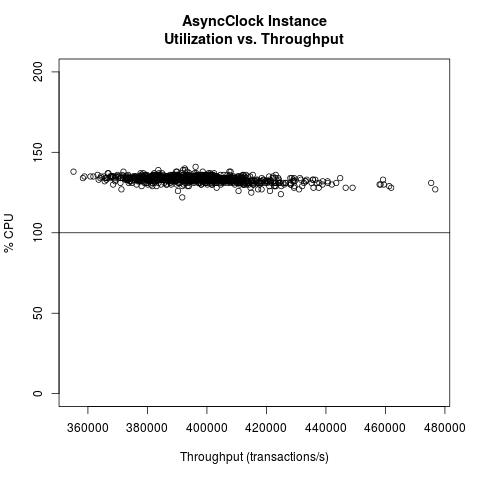
\includegraphics[height=.4\textheight]{async_instance_throughput_utilization.png}
\caption{\label{async_instance_throughput_utilization}}
\end{figure}

\begin{figure}
\center
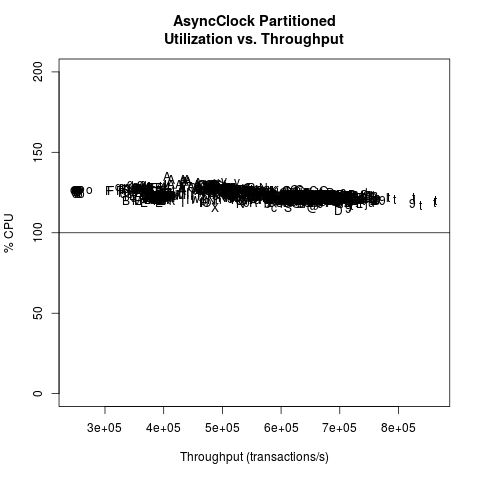
\includegraphics[height=.4\textheight]{async_partitioned_throughput_utilization.png}
\caption{\label{async_partitioned_throughput_utilization}}
\end{figure}

Figures~\ref{async_thread_throughput_context}, \ref{async_instance_throughput_context}, and \ref{async_partitioned_throughput_context} show plots of voluntary context switches versus throughput for Thread, Instance, and Partitioned, respectively.
Voluntary context switches include the situation where a thread blocks while waiting for a lock and is swapped out.
The Thread scheduler appears to have a consistently high number of context switches.
This is expected since there are three threads competing for two processors.
The Instance scheduler has fewer context switches and perhaps shows a slight trend where throughput increases with fewer context switches.
As previously stated, this is most likely the result of locking behavior.
The Partitioned scheduler shows a strong trend of throughput increasing with fewer context switches.
Furthermore, the partitions appear to cluster together.
For example, all of the runs for partition `o' of Table~\ref{async_partitions} appear in the upper left of Figure~\ref{async_partitioned_throughput_context}, while the runs for partition `t' appear in the lower right.
In partition `o', thread 0 contains System, Counter, Tick, Request, and Response while thread 1 contains Server and Client.
This mapping serializes the execution (Request, Response, and Tick are on one thread) and is subject to contention arising from the Server and Client garbage collection actions competing with Request and Response.
In partition `t', thread 0 contains System, Counter and Tick while thread 1 contains Server, Client, Response, and Request.
The only contention in this mapping is between Response on thread 1 and Counter and Tick on thread 0.

\begin{figure}
\center
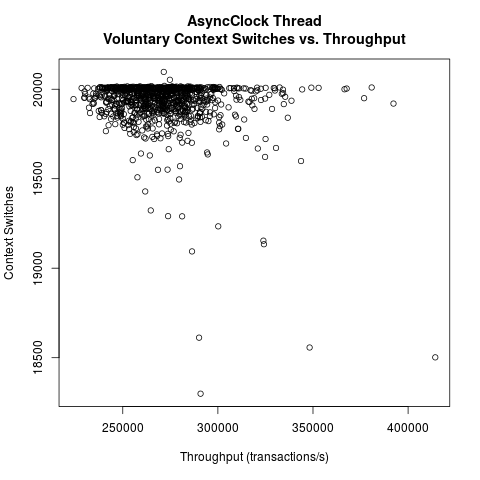
\includegraphics[height=.4\textheight]{async_thread_throughput_context.png}
\caption{\label{async_thread_throughput_context}}
\end{figure}

\begin{figure}
\center
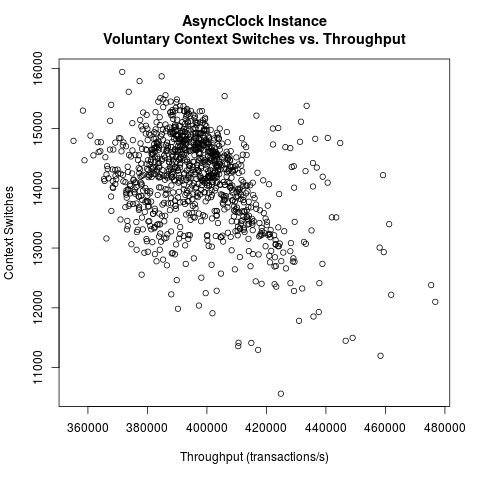
\includegraphics[height=.4\textheight]{async_instance_throughput_context.png}
\caption{\label{async_instance_throughput_context}}
\end{figure}

\begin{figure}
\center
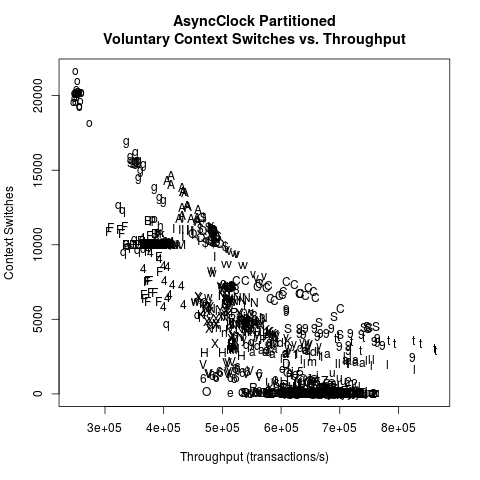
\includegraphics[height=.4\textheight]{async_partitioned_throughput_context.png}
\caption{\label{async_partitioned_throughput_context}}
\end{figure}

Figure~\ref{async_thread_throughput_entanglement} shows a plot of entanglement versus throughput for Thread.
The Thread scheduler has a minimum entanglement of 20,000 which is caused by the forced interleaving of the Request and Response threads and a maximum entanglement of 30,000.
Thus, the lowest band in Figure ~\ref{async_thread_throughput_entanglement} corresponds to no entanglement with the Tick thread.
In these cases, the Linux thread scheduler executes the Request/Response threads first and the Tick thread second (or vice versa).
The generally low entanglement shows that the Linux scheduler prefers to serialize the execution.
This is reasonable given that the Thread scheduler is subject to a performance hit caused by context switches as previously described.
The upper band suggests a bound on the allowed entanglement.
One explanation for this behavior is that the Linux scheduler may limit context switches, which has the effect of limiting the entanglement in the Thread scheduler.
Another explanation is that the entanglement may be limited based on the threads starting at different times.

Figure~\ref{async_instance_throughput_entanglement} shows a plot of entanglement versus throughput for the Instance scheduler.
The minimum entanglement is 0 and the maximum entanglement is 30,000\footnote{Let Transaction(Thread) indicate that the transaction was executed by the corresponding thread.  The following pattern when repeated 5,000 times generates an entanglement of 30,000:  Request(0) Tick(1) Response(0) Request(1) Tick (0) Response (1).}.
This plot does not appear to show a relationship between throughput and entanglement.

Figure~\ref{async_partitioned_throughput_entanglement} shows a plot of entanglement versus throughput for Partitioned.
This plot contains a band at 20,000 which contains roughly half of the samples (513/1000).
These correspond to arrangements where Request and Response are mapped to different execution threads which forces an entanglement of 20,000.
Half of the remaining samples have no entanglement (246/1000).
These correspond to arrangements where the Request, Response, and Tick are mapped to the same execution thread where no entanglement is possible.
The remaining quarter of the samples (241/1000) correspond to arrangements where Request and Response are on one execution thread while Tick is on the other.
These show varying degrees of entanglement with perhaps a slight trend toward increasing throughput with greater entanglement.
This is expected because the concurrency between Request and Tick can be exploited in these arrangements.

\begin{figure}
\center
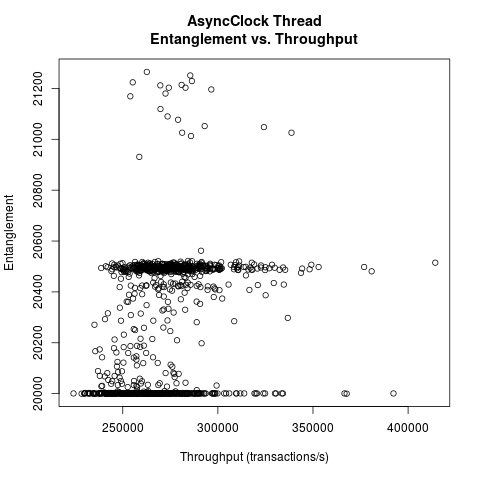
\includegraphics[height=.4\textheight]{async_thread_throughput_entanglement.png}
\caption{\label{async_thread_throughput_entanglement}}
\end{figure}

\begin{figure}
\center
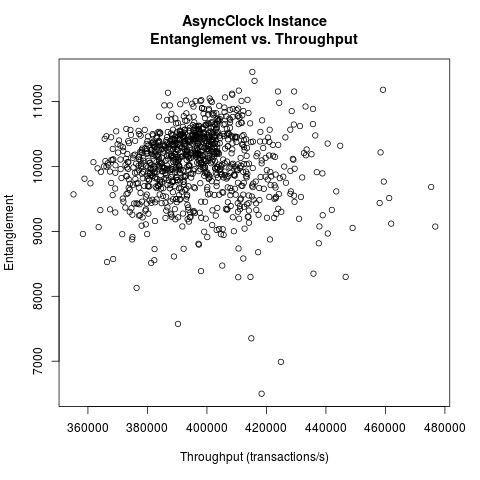
\includegraphics[height=.4\textheight]{async_instance_throughput_entanglement.png}
\caption{\label{async_instance_throughput_entanglement}}
\end{figure}

\begin{figure}
\center
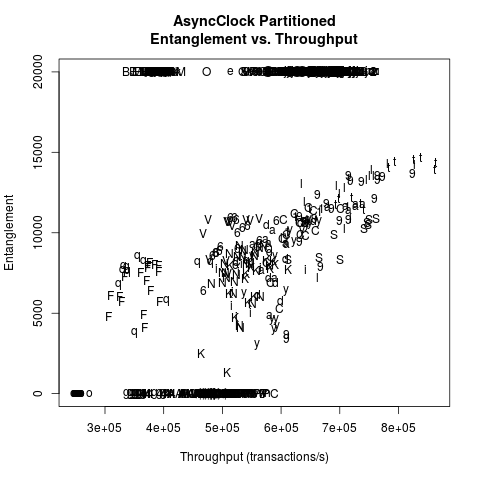
\includegraphics[height=.4\textheight]{async_partitioned_throughput_entanglement.png}
\caption{\label{async_partitioned_throughput_entanglement}}
\end{figure}

Figures~\ref{async_thread_latency}, \ref{async_instance_latency}, and \ref{async_partitioned_latency} show histograms of the latency for the Thread, Instance, and Partitioned schedulers, respectively.
All plots of latency use a logarithmic x-axis, as the latency distributions have very long tails.
For Thread, the mean latencies of the transactions are as follows:
\begin{center}
\begin{tabular}{cr}
Tick     &  .11769us \\
Request  & 5.30299us \\
Response & 5.63980us \\
\end{tabular}
\end{center}
Thus, the distribution on the left in Figure~\ref{async_thread_latency} corresponds to the latency of the Tick while the distribution on the right corresponds to the latency of Request and Response.
In the Thread scheduler, Tick transactions can be executed in quick succession as they are in a tight loop.
For the Instance scheduler, the mean latencies of the transactions are as follows:
\begin{center}
\begin{tabular}{cr}
Tick     & 5.22393us \\
Request  & 2.83083us \\
Response & 2.58799us \\
\end{tabular}
\end{center}
The Instance scheduler tends to serialize the execution of transactions for AsyncClock due to race conflicts.
Thus, Tick has roughly twice the latency of Request and Response since Tick is always enabled while Request and Response are enabled by each other.
For Partitioned, the mean latencies of the transactions are as follows:
\begin{center}
\begin{tabular}{cr}
Tick     & 2.49278us \\
Request  & 2.31450us \\
Response & 2.06478us \\
\end{tabular}
\end{center}
The work-conserving nature of the Partitioned scheduler allows it to achieve a lower average latency for all transactions when compared to the Instance scheduler.

\begin{figure}
\center
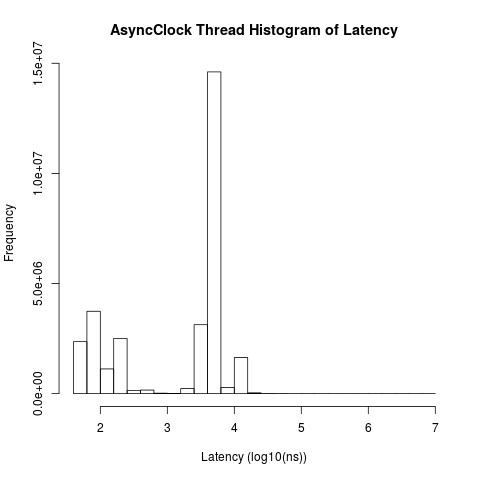
\includegraphics[height=.4\textheight]{async_thread_latency_hist.png}
\caption{\label{async_thread_latency}}
\end{figure}

\begin{figure}
\center
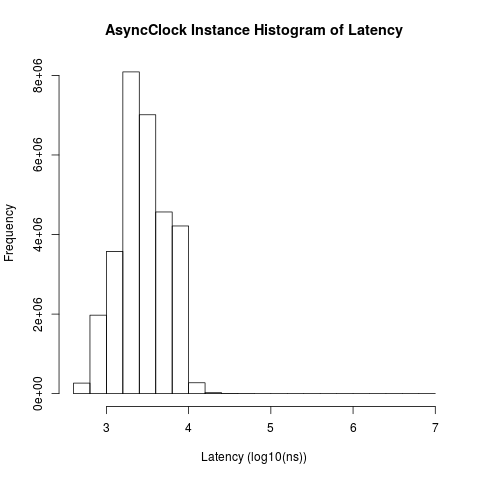
\includegraphics[height=.4\textheight]{async_instance_latency_hist.png}
\caption{\label{async_instance_latency}}
\end{figure}

\begin{figure}
\center
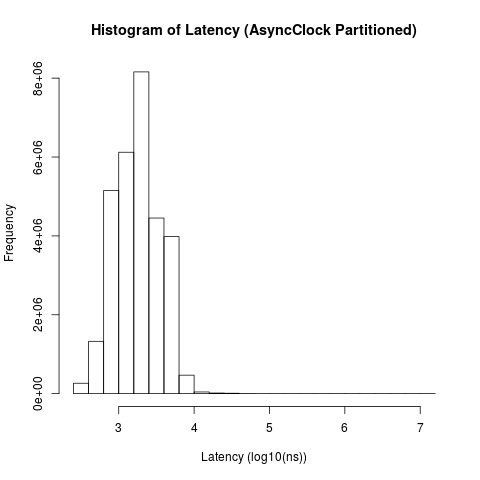
\includegraphics[height=.4\textheight]{async_partitioned_latency_hist.png}
\caption{\label{async_partitioned_latency}}
\end{figure}

Figure~\ref{async_throughput_box} shows a box plot of the throughput for the Thread, Instance, and Partitioned schedulers.
The quantiles of the throughput in transactions/s for each scheduler are as follows:
\begin{center}
\begin{tabular}{crrrrr}
Scheduler   &       0\%   &    25\%     &    50\%     &    75\%     &   100\% \\
\hline
Partitioned &   246,370.0 &   472,679.2 &   576,411.0 &   664,042.5 &    862,717.0 \\
Instance    &   355,158.0 &   386,067.8 &   395,796.0 &   405,083.8 &    476,759.0 \\
Thread      &   224,107.0 &   256,876.0 &   269,193.5 &   282,329.0 &    414,293.0 \\
\end{tabular}
\end{center}
The work-conserving nature of the Partitioned scheduler allows it to achieve a higher throughput than the Instance scheduler, and its ability to avoid context switches allows it to achieve a higher throughput than the Thread scheduler.
However, the figure and table also demonstrate the variability in the throughput due to the many modes of partitioning.
Thus, the Partitioned scheduler could be improved by using the race graph to avoid ``bad'' partitions.

\begin{figure}
\center
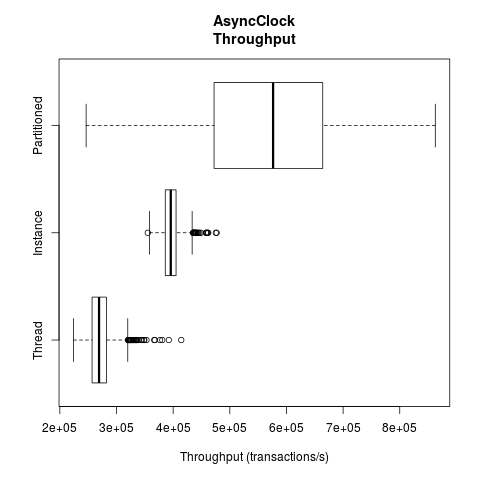
\includegraphics[height=.4\textheight]{async_throughput_box.png}
\caption{\label{async_throughput_box}}
\end{figure}

Figure~\ref{async_latency_box} shows a box plot of the latency for the Thread, Instance, and Partitioned schedulers.
The quantiles of the latency (in ns) for each scheduler are as follows:
\begin{center}
\begin{tabular}{crrrrr}
Scheduler &       0\%  &    25\%  &    50\%  &    75\%  &   100\% \\
\hline
Partitioned & 293 & 1,075 & 1,754 & 2,861 & 10,296,400 \\
Instance    & 423 & 1,851 & 2,645 & 4,569 &  8,028,100 \\
Thread      &  52 &   160 & 4,352 & 5,051 &  7,791,400 \\
\end{tabular}
\end{center}
The Thread scheduler achieves the lowest latency via the Tick transaction due to its work-conserving nature and optimized locking scheme.

\begin{figure}
\center
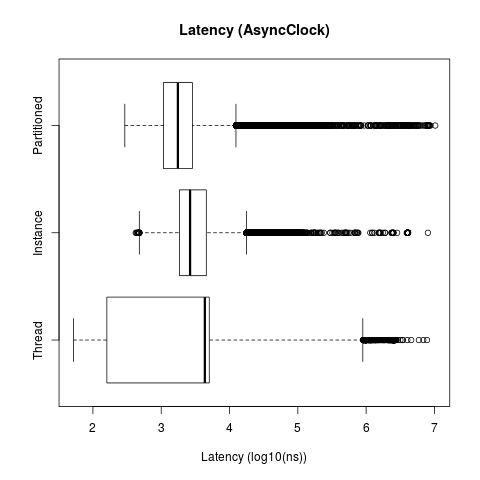
\includegraphics[height=.4\textheight]{async_latency_box.png}
\caption{\label{async_latency_box}}
\end{figure}

Both the Instance and Partitioned schedulers contain transactions for performing garbage collection.
These transactions do not actually perform any work since none of the transactions in the AsyncClock system allocate memory.
The Instance scheduler executed an average of 33,053 garbage collection actions per run while the Partitioned scheduler executed an average of 97,078 garbage collection actions per run.
The excessive number of collections performed by the Partitioned scheduler show a potential problem between the garbage-collection-as-an-action idea and work conserving schedulers as a work conserving scheduler can always find more work in garbage collection.
Ideally, a scheduler would be designed to not even select a garbage collection action until it has a high probability of actually collecting garbage.

\clearpage

\paragraph{SyncClock results.}
Figures~\ref{sync_thread_throughput}, \ref{sync_instance_throughput}, and \ref{sync_partitioned_throughput} show histograms of the throughput for Thread, Instance, and Partitioned, respectively.
The throughput curves of the Thread and Instance schedulers appear to be combinations of two or three distributions.
Like the AsyncClock experiment, the throughput for the Partitioned scheduler is a mixture of distributions arising from different partitioning schemes.
In the SyncClock system, there are two components and two transactions resulting in 8 possible partitions.
The list of partitions is given in Table~\ref{sync_partitions}.

\begin{figure}
\center
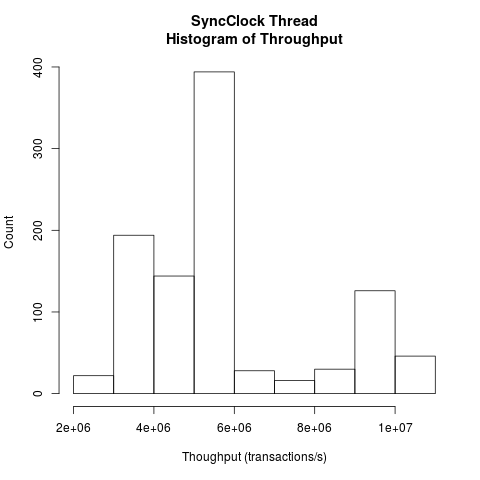
\includegraphics[height=.4\textheight]{sync_thread_throughput_hist.png}
\caption{\label{sync_thread_throughput}}
\end{figure}

\begin{figure}
\center
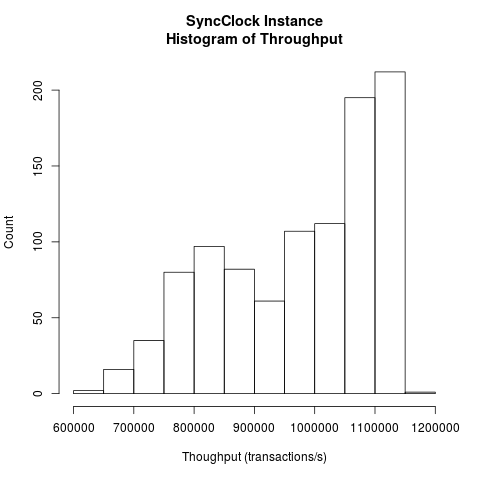
\includegraphics[height=.4\textheight]{sync_instance_throughput_hist.png}
\caption{\label{sync_instance_throughput}}
\end{figure}

\begin{figure}
\center
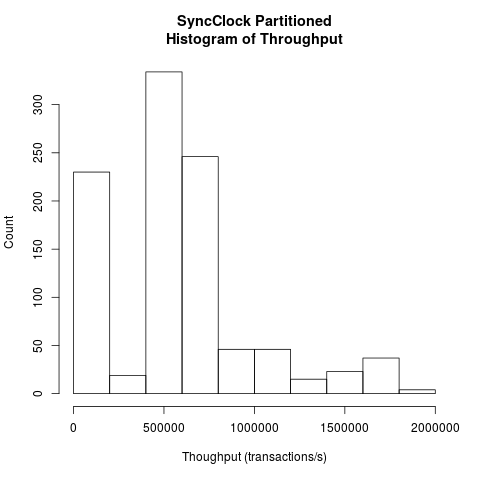
\includegraphics[height=.4\textheight]{sync_partitioned_throughput_hist.png}
\caption{\label{sync_partitioned_throughput}}
\end{figure}

Figures~\ref{sync_thread_throughput_utilization}, \ref{sync_instance_throughput_utilization}, and \ref{sync_partitioned_throughput_utilization} show plots of utilization versus throughput for the Thread, Instance, and Partitioned schedulers, respectively.
The utilization for the Thread scheduler decreases with increasing throughput.
This suggests that the Linux scheduler is serializing the execution of the threads which decreases utilization while avoiding lock contention which results in increased throughput.
Most of the runs for the Instance scheduler and Partitioned scheduler achieve a utilization greater than 100\% while a number of runs for the Thread scheduler do not.
The Instance scheduler shows a weak trend of increased utilization with throughput while the Partitioned scheduler shows a trend of decreased utilization with throughput.

\begin{figure}
\center
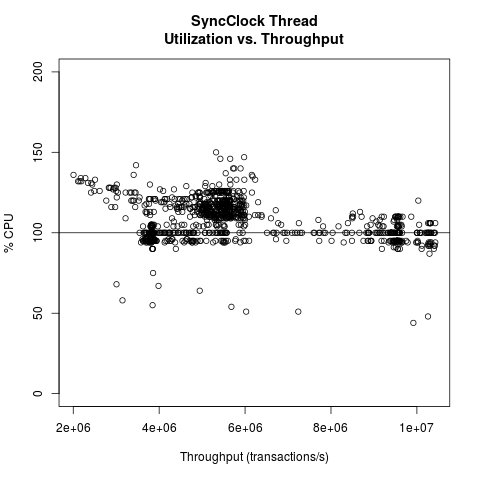
\includegraphics[height=.4\textheight]{sync_thread_throughput_utilization.png}
\caption{\label{sync_thread_throughput_utilization}}
\end{figure}

\begin{figure}
\center
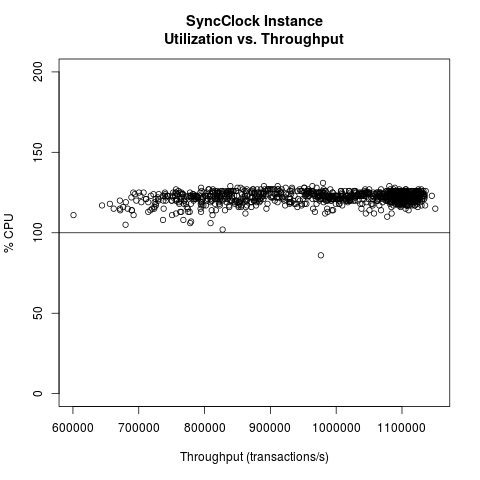
\includegraphics[height=.4\textheight]{sync_instance_throughput_utilization.png}
\caption{\label{sync_instance_throughput_utilization}}
\end{figure}

\begin{figure}
\center
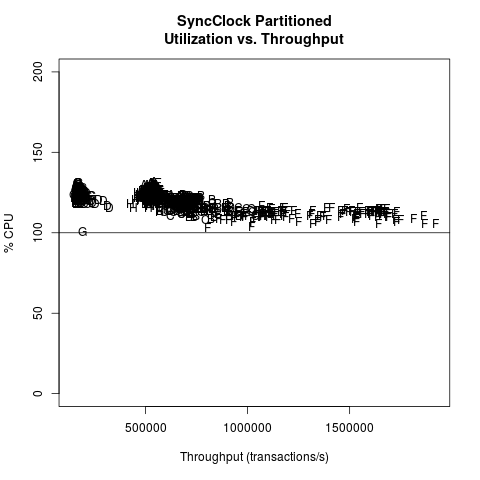
\includegraphics[height=.4\textheight]{sync_partitioned_throughput_utilization.png}
\caption{\label{sync_partitioned_throughput_utilization}}
\end{figure}

Figures~\ref{sync_thread_throughput_context}, \ref{sync_instance_throughput_context}, and \ref{sync_partitioned_throughput_context} show plots of voluntary context switches versus throughput for the Thread, Instance, and Partitioned schedulers, respectively.
All show a trend where throughput increases with decreasing context switches.
Both the Thread and Instance schedulers have a threshold where high throughput appears to require minimizing the number of context switches.
The plot for the Partitioned scheduler clearly shows an inverse relationship between throughput and context switches.

\begin{figure}
\center
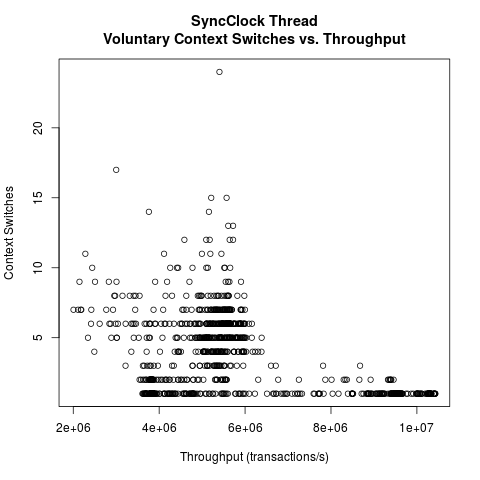
\includegraphics[height=.4\textheight]{sync_thread_throughput_context.png}
\caption{\label{sync_thread_throughput_context}}
\end{figure}

\begin{figure}
\center
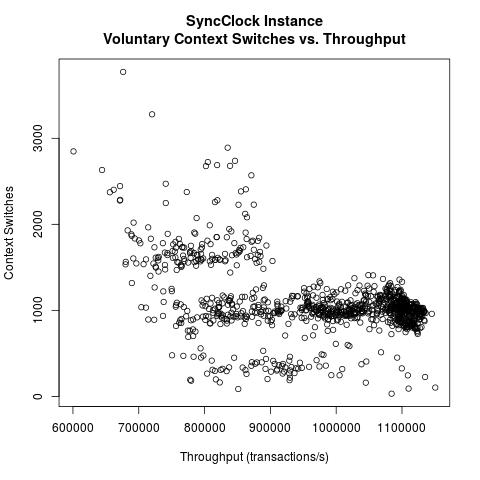
\includegraphics[height=.4\textheight]{sync_instance_throughput_context.png}
\caption{\label{sync_instance_throughput_context}}
\end{figure}

\begin{figure}
\center
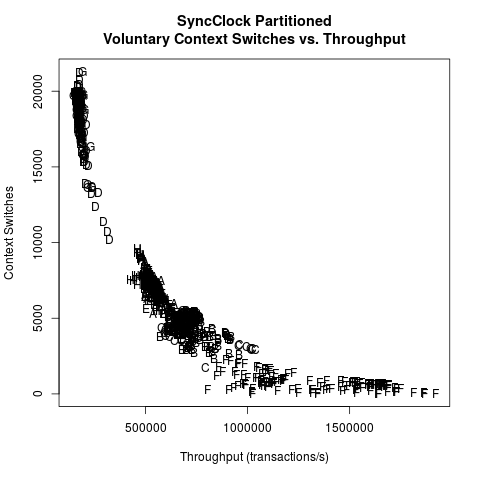
\includegraphics[height=.4\textheight]{sync_partitioned_throughput_context.png}
\caption{\label{sync_partitioned_throughput_context}}
\end{figure}

Figures~\ref{sync_thread_throughput_entanglement}, \ref{sync_instance_throughput_entanglement}, and \ref{sync_partitioned_throughput_entanglement} show plots of entanglement versus throughput for the Thread, Instance, and Partitioned schedulers, respectively.
The maximum entanglement for SyncClock is 20,000.
The plot of entanglement for the Thread scheduler resembles the plots of utilization and context switches.
The samples appear to be divided between concurrent (high entanglement, high context switch) and serial executions (low entanglement, low context switch).
For this system, it seems that it is more efficient to serialize the execution of the threads than to execute the threads concurrently and suffer context switches.

The plot of entanglement for the Instance scheduler shows a different trend where throughput increases with entanglement.
Thus, the Instance scheduler achieves high throughput when execution alternates between the threads without context switches.
The entanglement for the Partitioned scheduler appears to be a combination of three distributions.
The vertical line on the left consists of samples from the `G' partition which has maximal inter-thread conflicts and minimal opportunities for concurrent execution.
The horizontal line on the bottom (no entanglement) consists of samples from the `A', `D', `E', and `H' partitions which map Tick and Request to the same thread.
The execution is serialized with varying degrees of interference from the garbage collection actions.
The other samples contain the `B', `C', and `F' partitions which appear to show increasing throughput with entanglement.
The `F' partition has minimal inter-thread conflicts with maximal opportunities for concurrent execution.

\begin{figure}
\center
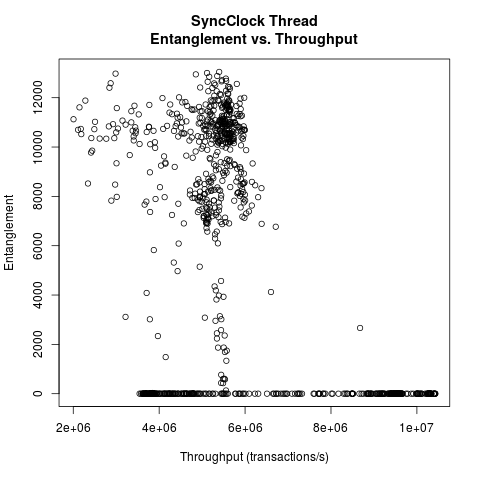
\includegraphics[height=.4\textheight]{sync_thread_throughput_entanglement.png}
\caption{\label{sync_thread_throughput_entanglement}}
\end{figure}

\begin{figure}
\center
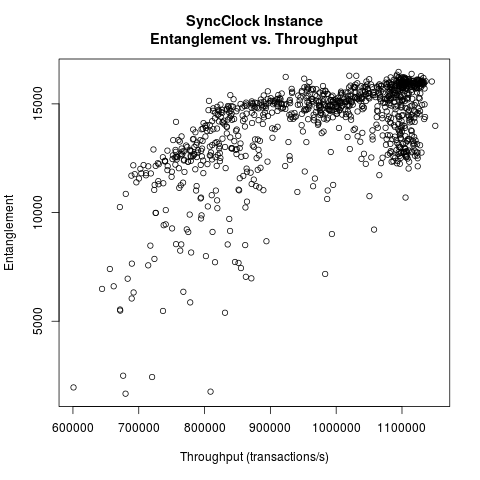
\includegraphics[height=.4\textheight]{sync_instance_throughput_entanglement.png}
\caption{\label{sync_instance_throughput_entanglement}}
\end{figure}

\begin{figure}
\center
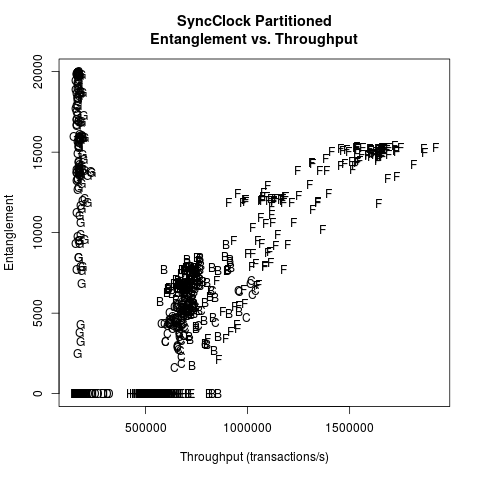
\includegraphics[height=.4\textheight]{sync_partitioned_throughput_entanglement.png}
\caption{\label{sync_partitioned_throughput_entanglement}}
\end{figure}

Figures~\ref{sync_thread_latency}, \ref{sync_instance_latency}, and \ref{sync_partitioned_latency} show histograms of the latency for the Thread, Instance, and Partitioned schedulers, respectively.
All plots of latency use a logarithmic x-axis, as the latency distributions have very long tails.
For the Thread scheduler, the mean latencies of the transactions are as follows:
\begin{center}
\begin{tabular}{cr}
Request &  72.952ns \\
Tick    & 207.145ns \\
\end{tabular}
\end{center}
The Request action does nothing more than acquire and release a lock which may explain its reduced latency.
For the Instance scheduler, the mean latencies of the transactions are as follows:
\begin{center}
\begin{tabular}{cr}
Request & 1,085.32ns \\
Tick    & 1,070.57ns \\
\end{tabular}
\end{center}
For the Partitioned scheduler, the mean latencies of the transactions are as follows:
\begin{center}
\begin{tabular}{cr}
Request & 4,117.71ns \\
Tick    & 4,069.06ns \\
\end{tabular}
\end{center}

\begin{figure}
\center
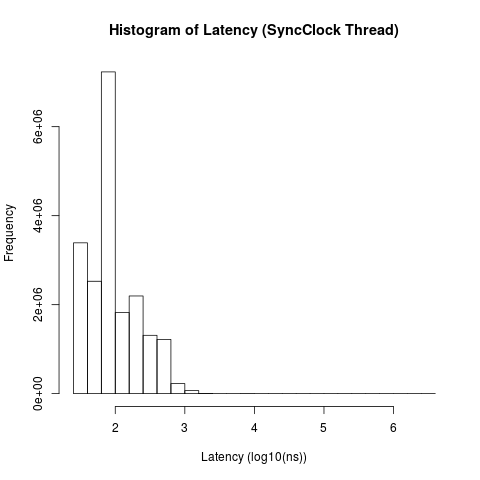
\includegraphics[height=.4\textheight]{sync_thread_latency_hist.png}
\caption{\label{sync_thread_latency}}
\end{figure}

\begin{figure}
\center
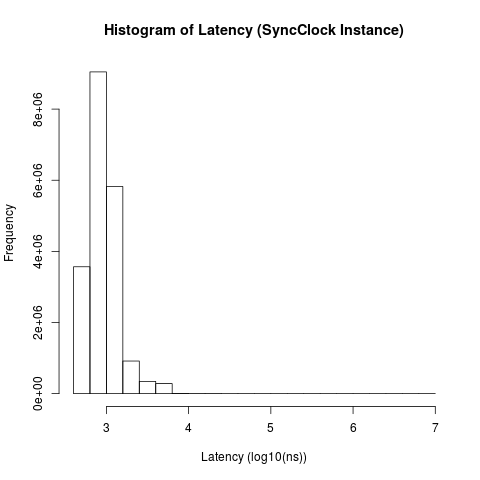
\includegraphics[height=.4\textheight]{sync_instance_latency_hist.png}
\caption{\label{sync_instance_latency}}
\end{figure}

\begin{figure}
\center
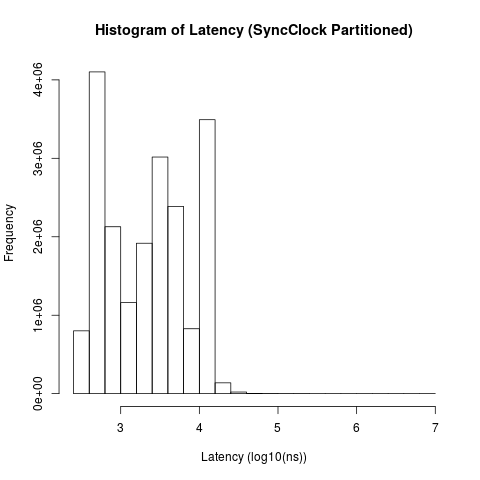
\includegraphics[height=.4\textheight]{sync_partitioned_latency_hist.png}
\caption{\label{sync_partitioned_latency}}
\end{figure}

Figure~\ref{sync_throughput_box} shows a box plot of the throughput for the Thread, Instance, and Partitioned schedulers.
The quantiles of the throughput in transactions/s for each scheduler are as follows:
\begin{center}
\begin{tabular}{crrrrr}
Scheduler   &       0\%   &    25\%     &    50\%     &    75\%     &   100\% \\
\hline
Partitioned &   146,788.0 &   439,051.0 &   558,954.5 &   711,073.8 &  1,919,680.0 \\
Instance    &   600,871.0 &   862,315.8 & 1,007,265.0 & 1,095,980.0 &  1,150,600.0 \\
Thread      & 2,005,940.0 & 4,308,048.0 & 5,382,440.0 & 5,983,532.0 & 10,428,200.0 \\
\end{tabular}
\end{center}
The Thread scheduler is clearly the best in terms of throughput.
The better performing partitions of the Partitioned scheduler are able to achieve the low end performance of the Thread scheduler.
In aggregate, however, the Instance scheduler appears to be better than the Partitioned scheduler.

\begin{figure}
\center
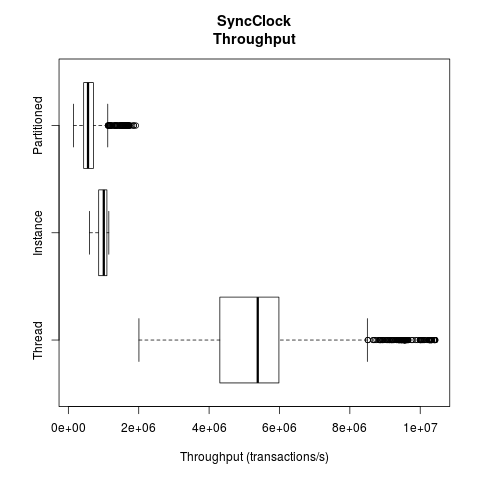
\includegraphics[height=.4\textheight]{sync_throughput_box.png}
\caption{\label{sync_throughput_box}}
\end{figure}

Figure~\ref{sync_latency_box} shows a box plot of the latency for the Thread, Instance, and Partitioned schedulers.
The quantiles of the latency (in ns) for each scheduler are as follows:
\begin{center}
\begin{tabular}{crrrrr}
Scheduler &       0\%  &    25\%  &    50\%  &    75\%  &   100\% \\
\hline
Partitioned & 293 &   636 & 2,469 & 4,835 &  8,100,990 \\
Instance    & 442 &   668 &   798 & 1,254 &  8,029,550 \\
Thread      &  27 &    59 &    80 &   160 &  2,736,960 \\
\end{tabular}
\end{center}
The Thread scheduler has the best latency by an order of magnitude.
This is unsurprising given the efficiency of the Thread implementation.

\begin{figure}
\center
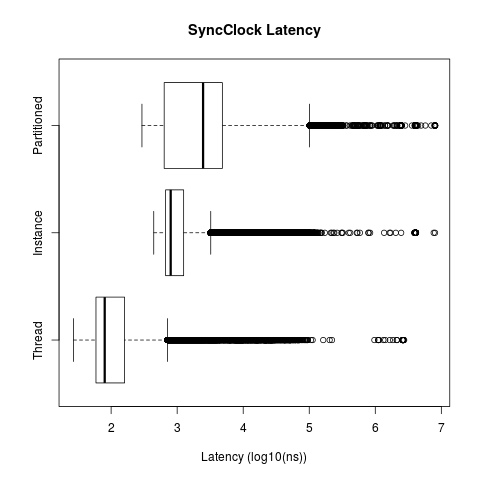
\includegraphics[height=.4\textheight]{sync_latency_box.png}
\caption{\label{sync_latency_box}}
\end{figure}

\clearpage

\section{Conclusions and Future Work}

The goal of implementing reactive components was to test the practicality of the reactive component model.
Specifically, we desired to know how the various features of the model could be implemented, which features were troublesome, and how the implementation utilizes various assumptions.
Flexibility in the reactive component model necessitates a check for sound composition.
The sound composition algorithm described in this chapter uses the static system assumption and the component proxy assumption to generate a graphical model of each transition and check it for determinism.
A cursory analysis yielded an upper bound of $O(k n^2 \log (n))$ where $n$ is the number of instances involved in the transaction.

To implement activation statements, we developed the synchronized two-phase calling convention which executes the immutable phase of a transaction in the first phase and preserves the context necessary for the second phase which corresponds to the mutable phase.
The synchronized two-phase calling convention was implemented using standard function call and stack manipulation facilities.

The isolation of component state is enforced in two ways.
First, the type system prevents components from sharing pointers directly via \verb+$const+ and \verb+$foreign+ modifiers.
Second, the implementation uses garbage collection to prevent indirect sharing through dangling pointers.
In this chapter, we describe the implementation of heaps and how they are used for dynamic memory allocation.
Heaps are designed so that they can be merged and moved.
At the user level, all references to a heap are concentrated into a ``link'' which is used to enforce atomic moves and merges.
The independence of state between components allows each component to have its own heap (or tree of heaps) that can be garbage collected independently of other components.
Garbage collection can be conducted in parallel by associating a garbage collection action with each component.

To enhance the practicality of the reactive component implementation, we introduced file descriptor I/O that allows reactive components to interact with a variety of operating system facilities.
All I/O is non-blocking to preserve the fairness of the scheduler.
Components may use the \verb+readable+ and \verb+writable+ functions to test file descriptors.
The scheduler uses these functions as part of the termination protocol to sleep while waiting for external inputs.
File descriptors are treated as component state and therefore cannot be shared between components or mutated during the immutable phase.
Using file descriptor I/O, we implemented an SNTP client which demonstrates how systems can be built up from simple components.

Perhaps the most interesting part of the implementation is the scheduler.
Fairness, safety, and responsibility are identified as the three correctness requirements for any scheduler and we illustrate how these may be accomplished in a variety of designs.
Two multi-threaded schedulers were implemented.
The Instance scheduler is based on a shared work queue of instances while the Partitioned scheduler is based on partitioning transactions among different scheduler threads.
We propose throughput, latency, and utilization as three metrics for evaluating schedulers for reactive components and collected these metrics for the Instance and Partitioned schedulers by executing the AsyncClock and SyncClock systems.
The reactive component schedulers were compared to custom implementations of the same systems using the pthreads library.
%% The results show that the reactive component schedulers are viable as event schedulers but will require improvement to become competitive with threads.
%% Moving from interpretation to compilation, reducing locking overhead, and reducing the overhead of precondition evaluation seem to be promising areas for improvement.

The AsyncClock and SyncClock experiments demonstrate both the viability of reactive components as an event system and that more work is necessary to improve the design and implementation of the run-time system.
The motivation for events was to facilitate (logical) concurrency while avoiding the overhead of context switching associated with assigning each task to a thread.
The performance of the Partitioned scheduler over the Thread implementation of AsyncClock demonstrates this idea.
As was previously mentioned, events can be combined with multi-threading but care must be taken to ensure proper synchronization.
In the reactive component model, the burden of correct synchronization is placed on the scheduler instead of the developer.

The AsyncClock system is illustrative in that it shows the advantage of events over threads but is nevertheless unrealistic as it intentionally overloads the system.
The SyncClock system represents a scenario in which there are adequate resources for each thread.
In this situation, the Instance and Paritioned schedulers perform an order of magnitude worse than the Thread implementation.
This prompts the question:  can reactive components be as efficient as threads?
While we cannot answer this question definitively, the act of converting a reactive component program to a threaded program does provide evidence that it may be possible to make reactive components as efficient as threads.
The procedure for converting a reactive component program to a threaded program involves 1) creating a reader/writer lock for each component instance, 2) creating a thread for each transaction, 3) creating a condition variable and mutex for each precondition, 4) creating a critical section for each transaction, and 5) signaling affected transactions after the critical section.
It seems feasible that this procedure can be automated.
Thus, a system of reactive components can be converted to threads or scheduled as events depending on the resources available and nature of the transactions in the system, but doing so is left for future work.

There are three main areas that may be addressed to improve the performance of the Instance and Partitioned schedulers.
First, we may attempt to improve the efficiency of the schedulers through better design and implementation.
The evaluation in this section can serve as a basis for future improvements.
Second, we may attempt to eliminate the overhead of the Linux scheduler.
In Linux, the threads made available via the pthreads library are scheduled by the Linux kernel.
The Instance and Partitioned schedulers, then, are themselves scheduled by the Linux kernel.
Thus, it may be necessary to implement a scheduler for reactive components at the kernel level to eliminate this source of overhead.
Third, we may move from interpretation to compilation.
To test this idea, we timed a loop to sum the numbers in the range [0, 1,000,000) and averaged it over 1,000 runs for a C++ implementation and a reactive component implementation.
The average time for the reactive component implementation was 0.1304896 seconds and the average time for the C++ implementation was 0.0009984909 seconds; a speed-up factor of 131.
This is very much a ``back of the envelope'' calculation; the actual improvement in moving from interpretation to compilation may be less than this.

We selected the AsyncClock and SyncClock systems to evaluate the schedulers because they are small enough to understand but complex enough to show interesting behavior.
The actual computation performed by these systems is minimal, i.e., setting boolean flags and incrementing counters.
Most likely, these operations can be performed in a single clock cycle (for compiled programs).
One obvious direction for future work, then, is to experiment with complex transactions and varied workloads.
However, it is important to consider the possibility that real workloads will contain computationally simple transactions such as those found in the clock systems.
Furthermore, one of the motivations for decomposing systems is to break up complex systems into smaller, reusable, and easier to understand systems.
The results in this section demonstrate the diminishing return where the transactions become so simple that execution is dominated by overhead, i.e., it is more efficient to serialize execution than execute actions in parallel.
Simple transactions are a foreseeable consequence of decomposition and designers should not be penalized for decomposing complex systems.
Thus, one of the goals of scheduler design is to push the horizon of the diminishing return as far as possible.
When coupled with responsiveness, the desired property in a scheduler is one whose throughput does not diminish with entanglement.

One goal for a reactive component scheduler may be to optimize the evaluation of preconditions.
Two possible goals are to reduce the number of times a precondition is evaluated (lazy vs. eager) or to reduce the overhead of evaluating a single precondition.
The reactive component model allows arbitrary Boolean expressions to be used as preconditions.
One idea may be to eliminate preconditions and replace them with explicit scheduling instructions, but this may become tedious and error prone.
A compromise solution may involve restricting the complexity of preconditions to simple Boolean expressions, i.e., with no function calls.
With this restriction, it may become possible to determine which activation statements enable/disable a transaction.

To be safe, all concurrent schedulers require synchronization to protect the mutable state in a transaction.
The approach taken by the oblivious Instance and Partitioned schedulers is to acquire locks protecting the state of each involved component before executing a transaction.
The Partitioned scheduler demonstrates how asynchronous locking can be used to create a work-conserving scheduler.
As indicated by the results in this section, a major challenge is to make synchronization as efficient as possible.

Another direction for future work is to explore options that accomplish synchronization without locking or with minimal locking.
Partitioning combined with non-preemption may create opportunities to synchronize without locking.
Let $u$ be a transaction assigned to a specific scheduler thread and let $I$ be the set of instances involved in $u$.
Furthermore, let all transactions involving any component in $I$ be mapped to the same scheduler thread (the single-threaded schedulers described in this section do this by virtue of their design).
In this scenario, no locks are needed for a safe execution of $u$ because all other transactions that could change the relevant component state are excluded from executing due to the non-preemptive nature of the scheduler.
This phenomenon is illustrated graphically by coloring the nodes in an race graph according to the thread to which they have been assigned.
A transaction whose immediate neighbors all share the same color as the transaction itself can execute without acquiring locks.
This suggests that algorithms that detect clusters of transactions in the race graph may be used to optimize the assignment of transactions to scheduler threads.

Locking also may be optimized by performing operations on the race graph.
For example, adjacent transactions in the race graph can be merged and executed under the same set of locks.
This procedure can be used to create complex transactions that amortize the locking overhead.
Most likely, the merging algorithm would make use of some heuristic that measures the perceived benefit of merging the transactions.
For example, the edges in the race graph could be weighted with the Jacquard Index of the instance sets, i.e., the edges are weighted with a score indicating that the set of locks are similar.
The merging algorithm must balance the goal of simplifying the locking with the goal of exploiting concurrency.
For example, merging Request and Response eliminates the potential concurrency between Request and Tick in the \emph{AsyncClock} system.

Similarity between instance sets suggests the idea that locks may be eliminated by fusing them together.
To illustrate, the \emph{AsyncClock} system contains three locks corresponding to the three components.
Suppose that the same lock is used to protect both the Client and the Server.
This reduces the number of locks needed to execute the Request transaction from two to one and the number of locks needed to execute the Response transaction from three to two.

The challenges associated with locking invite us to step back and consider the fundamental aspects of the problem that necessitate a locking protocol.
The scheduler designs put forth so far are distributed in the sense that each scheduler thread is making an independent decision about the next transaction to execute.
Locking is the means by which the scheduler thread discovers the decisions made by the other scheduler threads to determine if the transaction under consideration is compatible with the transactions already chosen by the other threads.
The locking protocol becomes unnecessary if the decisions made by the other threads are already available, i.e., a knowledgeable scheduler.
This suggests that orchestration may be used to ensure safety in a multi-threaded scheduler without locking.
In this model, a manager thread assigns transactions to scheduler threads who execute the transactions without acquiring locks.
The primary job of the manager thread is to enforce safety by only allowing the concurrent execution of disconnected transactions in the race graph.
This approach may make use of a dedicated manager thread (Producer-Consumer) or use the Leader-Follower pattern~\cite{schmidt2000pattern}.
An efficient implementation of the scheduler state, especially if it is shared through the Leader-Follower pattern, is a concern for this kind of scheduler.
For systems with a fixed set of transactions, a compiler may be able to generate a scheduling automaton by enumerating the scheduler states $S$, pruning unsafe states and transitions according the rules outlined in section~\ref{scheduling_problem}, pruning transitions to ensure fairness, etc.
This formulation may have the advantage of yielding compact scheduler state.

Cache awareness and migration are two concerns that reactive component schedulers share with thread schedulers.
Cache awareness attempts to improve the performance of a system by scheduling a computation on the same processor core because the state required for the computation may already be available in the cache.
Thus, a reactive component scheduler may attempt to create an affinity between a transaction and a scheduler thread or processor core.
Partitioning on the basis of shared component state satisfies this implicitly.
Migration reassigns a computation to a different core to balance the load among the cores or free a core so that it may be shutdown.
The challenge with respect to migration is to define load imbalance in a meaningful way.
The migration algorithm will most likely be expressed as an optimization problem that attempts to find a global optimum for the throughput and latency of each action.

Another design dimension for a reactive component scheduler is preemption.
The main use of preemption is to share a physical core among many computations that are ready to execute.
A reactive component scheduler may wish to preempt a long-running transaction to execute other enabled transactions.
A preemptive scheduler for reactive components can take advantage of existing work on thread preemption.

%% POSIX environment, possibly bare metal

%% \item termination
%% \item active - terminating - idling (most servers have 10\% utilization)
%% \item flow control
%% \item always enabled actions
%% \item reactive components in hardware
%% \item long running actions
